\chapter{Pruebas} 
%\epigraph{\textit{I believe that at the end of the century the use of words and general educated opinion will have altered so much that one will be able to speak of machines thinking without expecting to be contradicted.     
%	}}{\textit{—  Alan Turing, Computing machinery and intelligence}}
%	\vspace*{8cm}
%	\begin{center}
%		\centering
%		\includegraphics[width=10.5cm]{example-image}
%	\end{center}
%	\thispagestyle{empty}
%	\newpage
\vspace*{2cm}

A lo largo de este capítulo se mostrarán las pruebas realizadas con el sistema obtenido, por cuestiones de tiempo se ha limitado el alcance esperado pero logrando el objetivo, realizar predicciones. Esto significa que se ejecuta en un entorno local y solo se mostrarán peticiones a la API desarrollada sin una aplicación con interfaz de usuario que la consuma. Aclarando lo anterior, iniciaremos con las pruebas a los puntos de acceso desarrollados en la API.

Las imagenes que se presentaran a lo largo de esta sección corresponden a peticiones realizadas con éxito mostrando los campos que necesita SISPREL para crear el elemento en la base de datos y al final se muestra la respuesta de SISPREL al crearlas.

\section{Pruebas de API}
En el capítulo pasado se ha descrito como funciona la documentación en la API, ya que estas pruebas se realizarán usando la herramienta generada por el sistema, para efectos prácticos se mostrarán las siguientes pruebas en este capítulo: \textit{creación de usuario abierto, inicio de sesión, crear encuesta, actualizar encuesta, crear pregunta, crear opción de pregunta y contestar pregunta}. Todos los puntos de acceso mencionados anteriormente exceptuando la creación de usuario abierto, están blindados con OAuth 2, no se puede hacer uso de estos a menos que se cuente con un token válido, si no, el sistema regresará un error 403 'No cuenta con los suficientes permisos'.


\subsection{Crear usuario abierto}
SISPREL permite el registro de usuarios nuevos sin necesidad de depender del administrador para crear dichos usuarios, en la figura \ref{graphic:TCUO} se puede muestra la petición con la respuesta de la API después de haber ingresado los datos solicitados por el punto de acceso correspondiente para el registro de un usuario, la cual nos genera un código 200 y nos devuelve el usuario creado en formato JSON.

\begin{figure}[!htb]
    \centering
    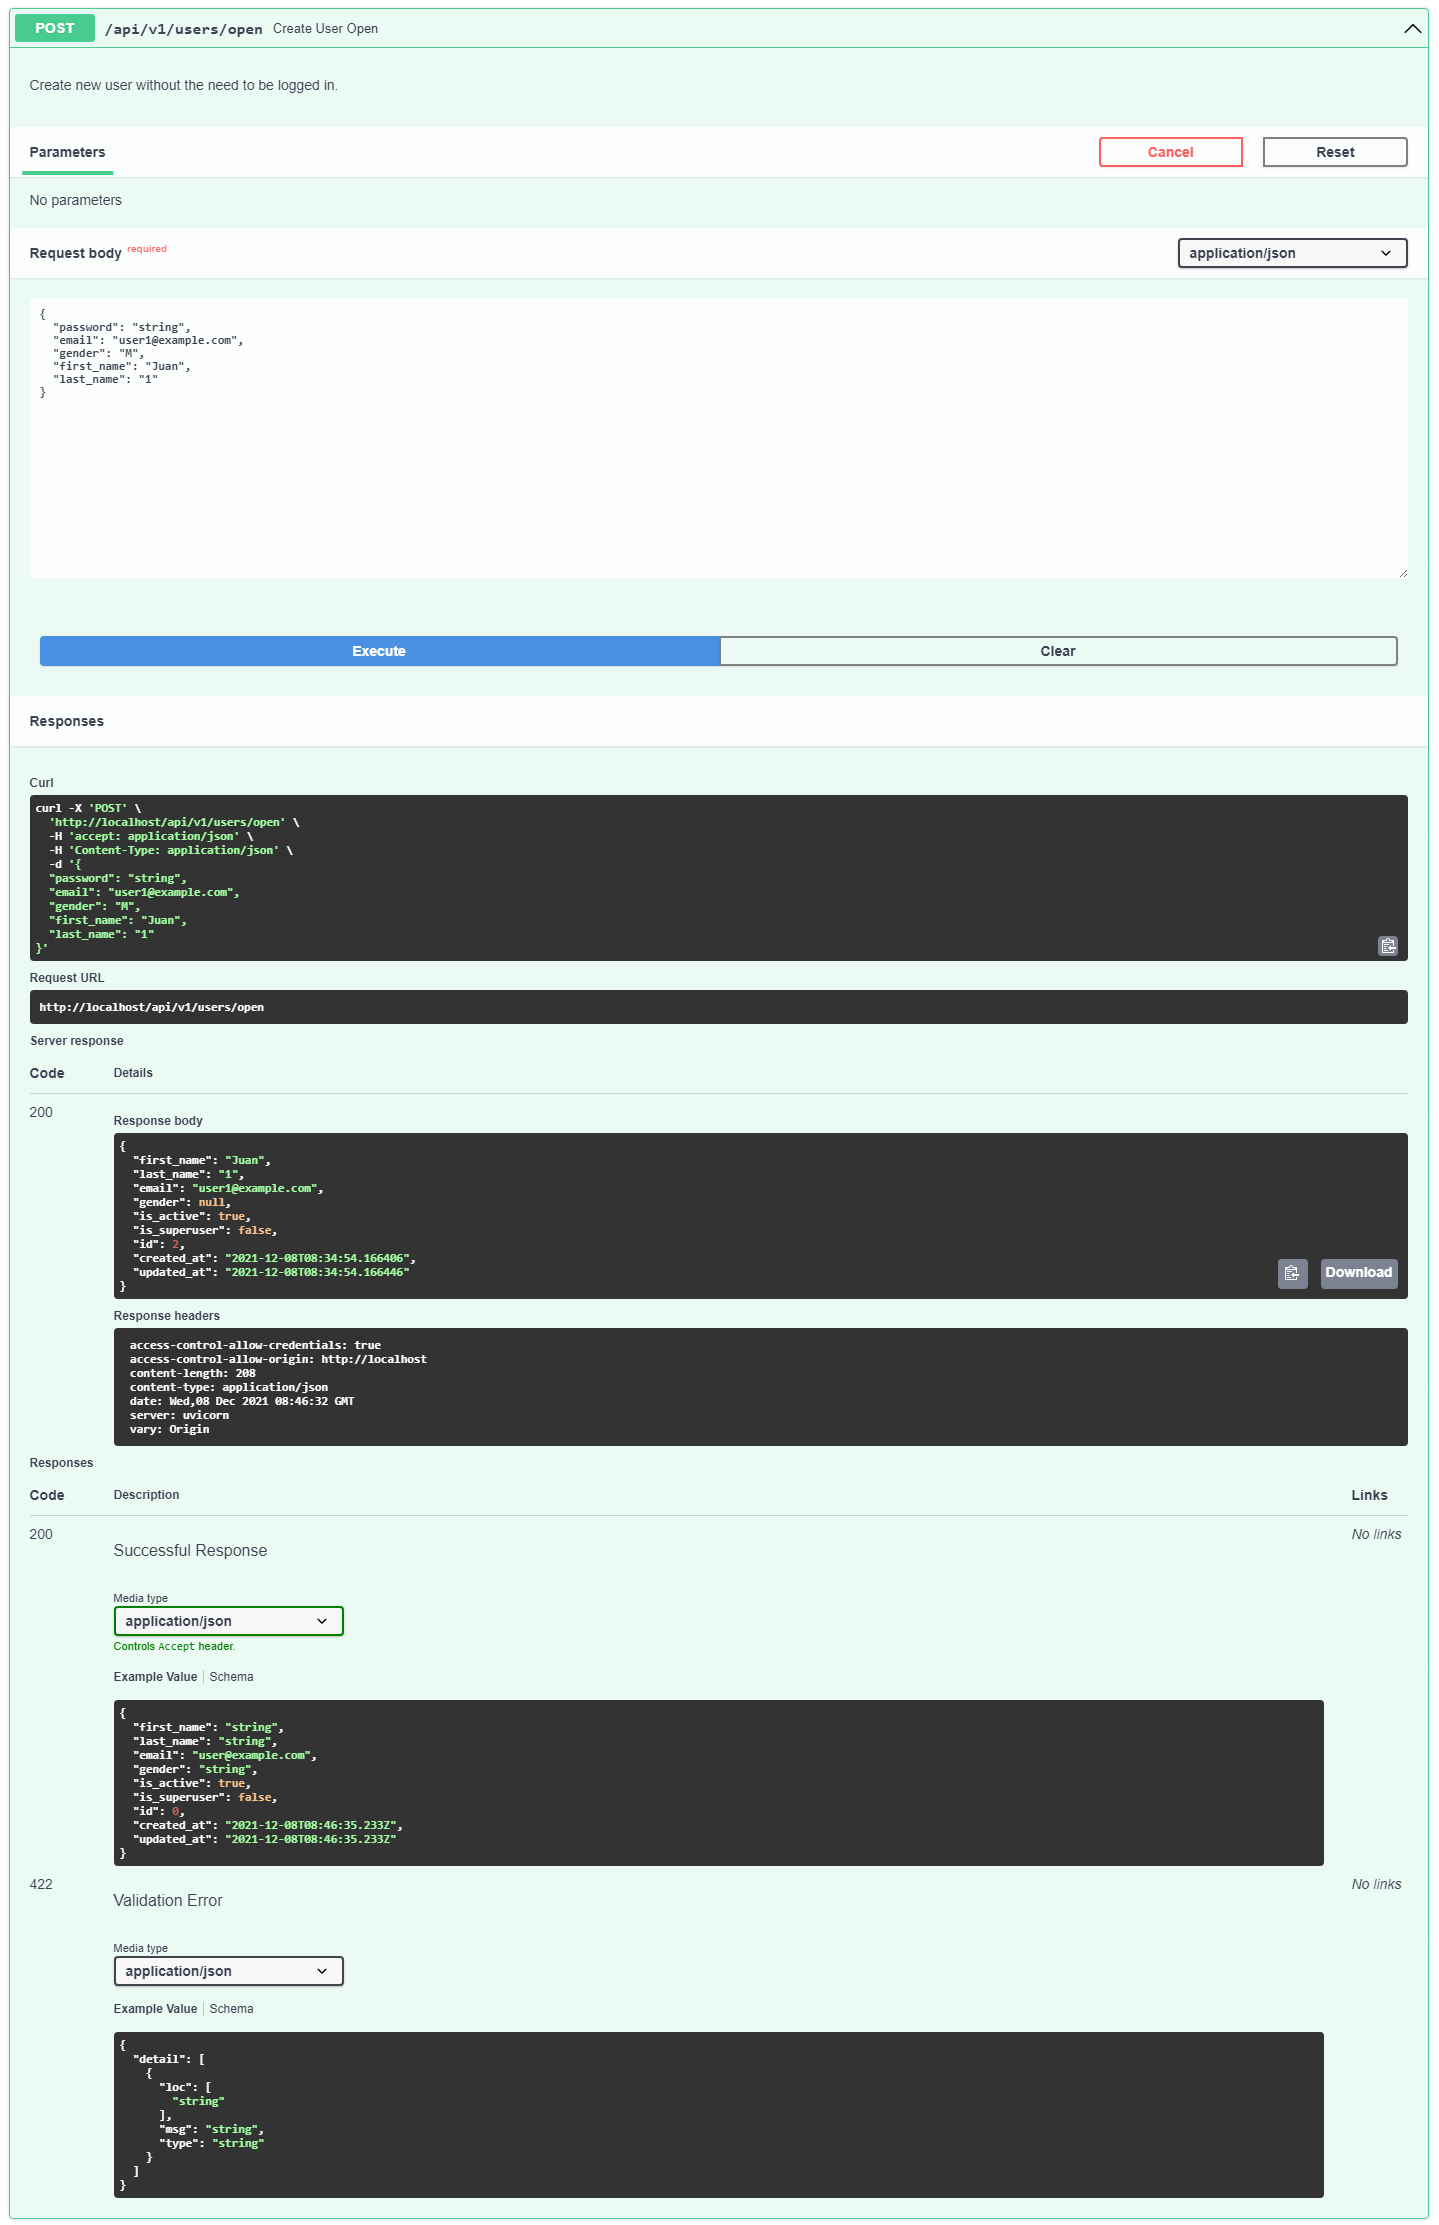
\includegraphics[scale=.275]{TT/img/pruebas/test_create_user_open.png}
    \caption{Creación de usuario abierto}
    \label{graphic:TCUO}
\end{figure}

\subsection{Iniciar sesión}
SISPREL usa la herramienta OAuth 2 para realizar los ingresos al sistema de manera segura, en la imagen \ref{graphic:iniciarsesion} se muestran los datos que se piden para iniciar sesión y en la imagen \ref{graphic:iniciodesesionexitoso} se puede apreciar el acceso al sistema, para este caso, iniciaremos sesión con la cuenta del administrador.

\begin{figure}[!htb]
    \centering
    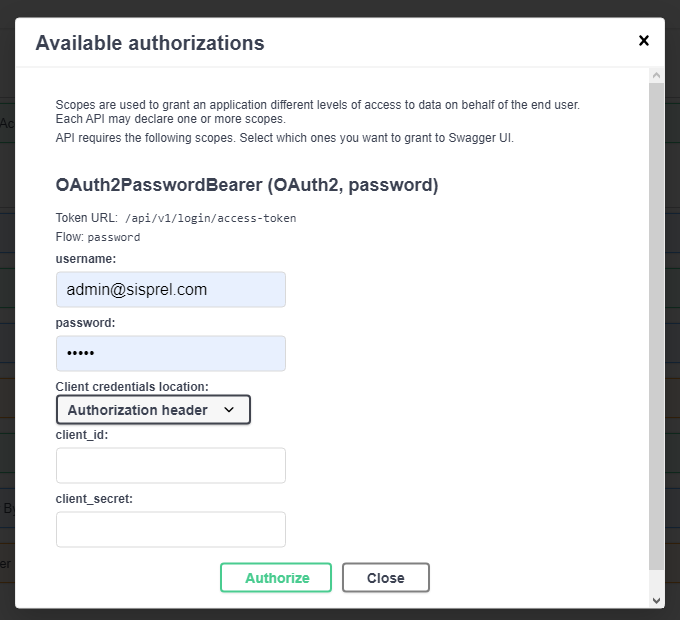
\includegraphics[scale=.5]{TT/img/pruebas/test_login_admin.png}
    \caption{Inicio de sesión}
    \label{graphic:iniciarsesion}
\end{figure}

\begin{figure}[!htb]
    \centering
    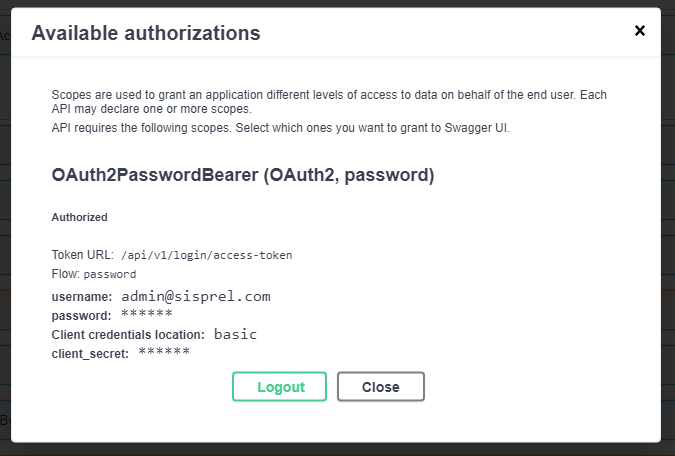
\includegraphics[scale=.5]{TT/img/pruebas/test_login_succesful.png}
    \caption{Inicio de sesión exitoso}
    \label{graphic:iniciodesesionexitoso}
\end{figure}

\subsection{Crear encuesta}
Lo siguiente a mostrar es la creación de una encuesta, para esto se ha dividido en dos partes, la primera consta de llenar los campos requeridos por SISPREL, y la segunda parte es cuando terminamos de crear todas las preguntas se procede a realizar una actualización de la encuesta, esto se debe a que para calcular el peso máximo total de una encuesta es necesario contar con todas las preguntas, ya sea que se eliminen o se crean mas preguntas es necesario repetir este peso, al menos en la primera versión de SISPREL.

En la imagen \ref{graphic:crearencuesta} se muestran los campos y la respuesta del sistema al crear una encuesta, algunos campos no son accesibles para el usuario, dado que el sistema se encarga de crearlos de manera automática o requiere de acciones extra para hacer algunos cálculos. El campo de preguntas regresa una lista vacía, esto es porque aun no hay preguntas asignadas a esta encuesta.

\begin{figure}[!htb]
    \centering
    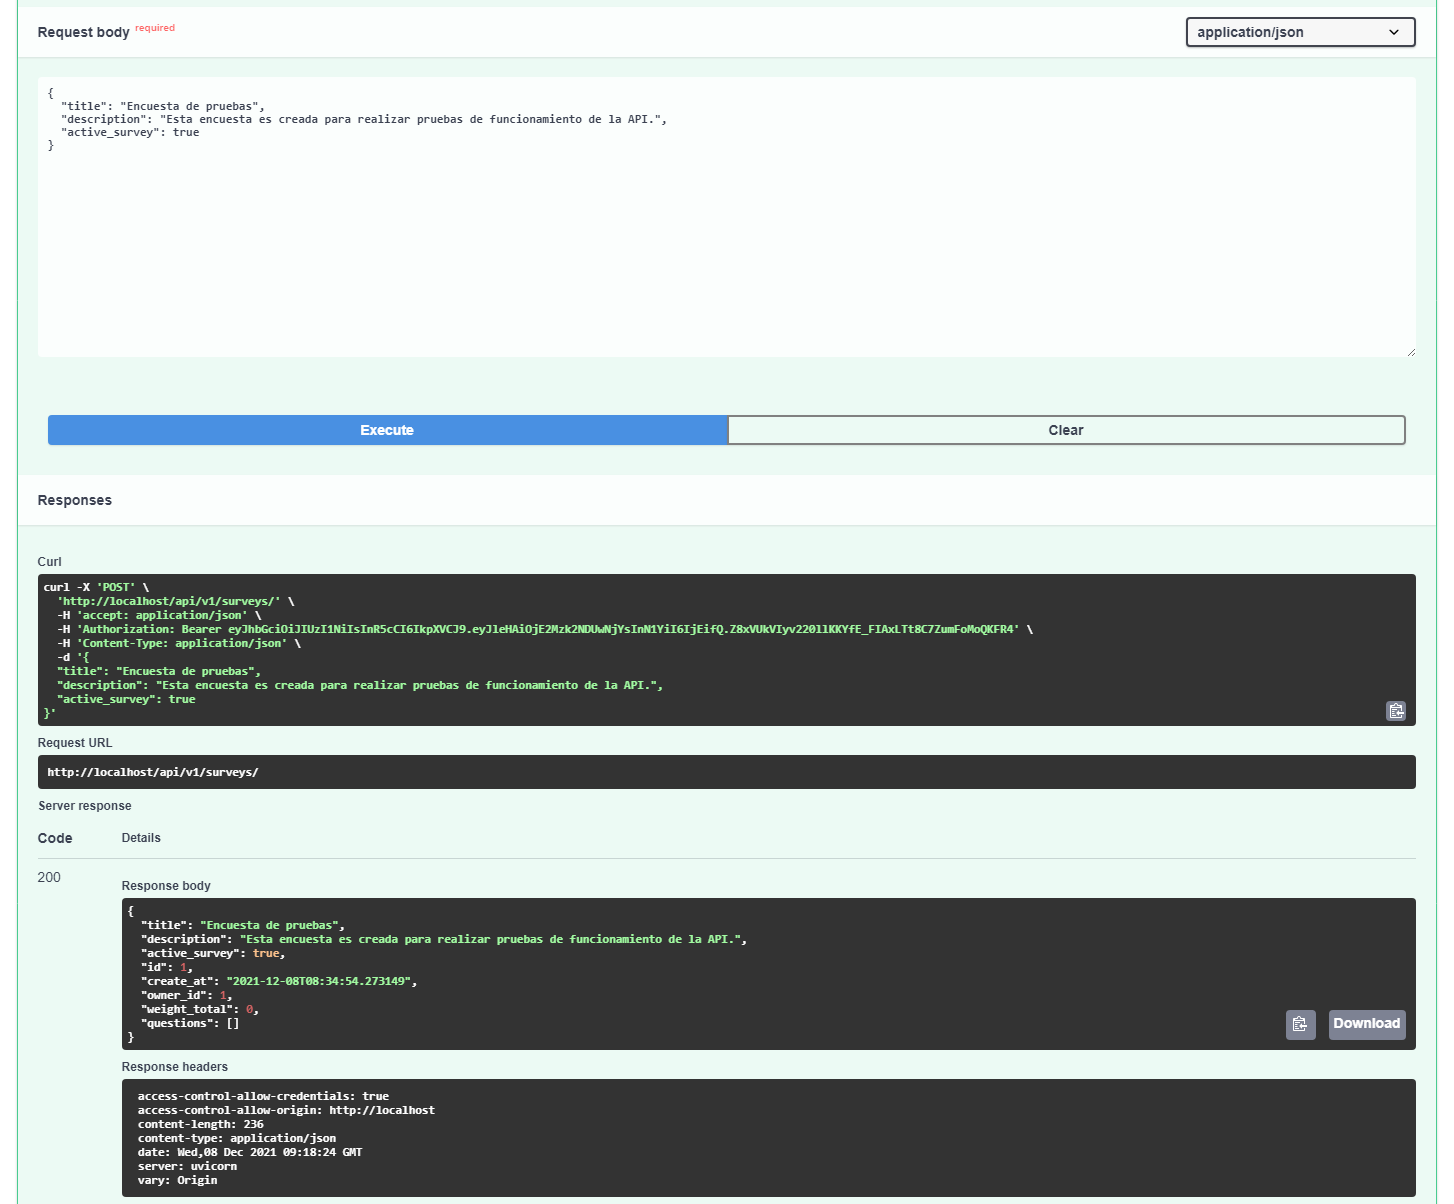
\includegraphics[scale=.3]{TT/img/pruebas/test_create_survey.png}
    \caption{Crear encuesta}
    \label{graphic:crearencuesta}
\end{figure}

\subsection{Crear pregunta}
En la imagen \ref{graphic:crearpregunta} se presenta los campos necesarios para crear una pregunta que pertenece a una pregunta, al inicio de la imagen SISPREL requiere de un parámetro para crear la pregunta, este parámetro es el ID de la encuesta a la cual será asignada. y al final de la imagen viene la respuesta de SISPREL cuando se crea una pregunta de manera exitosa, también devuelve un elemento que es una lista vacía, esto se debe a que aun no hay opciones de respuesta asignada en la pregunta.

\begin{figure}[!htb]
    \centering
    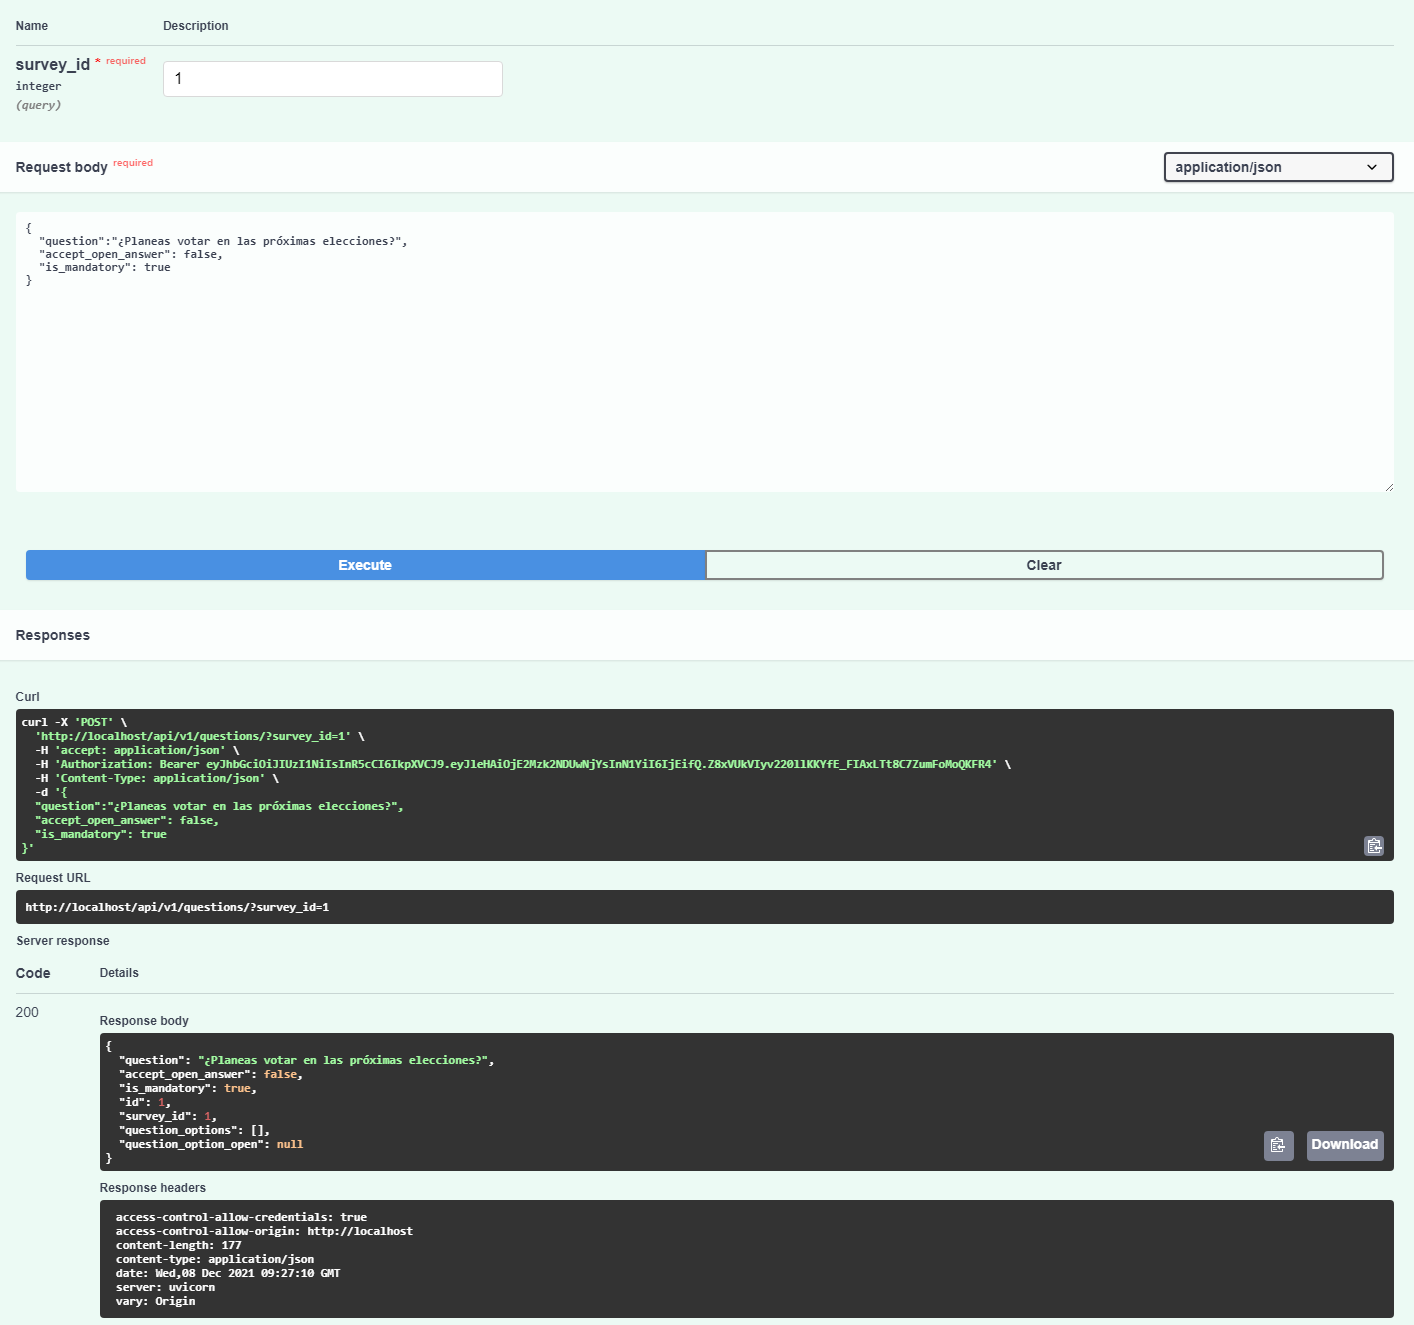
\includegraphics[scale=.3]{TT/img/pruebas/test_crear_pregunta.png}
    \caption{Crear pregunta}
    \label{graphic:crearpregunta}
\end{figure}

\subsection{Crear opción de respuesta}
En la imagen \ref{graphic:crearopcionderespuesta} se presenta los campos necesarios en el JSON y los parámetros (ID de encuesta e ID de pregunta) para crear una opción de respuesta asignada a una pregunta. 

\begin{figure}[!htb]
    \centering
    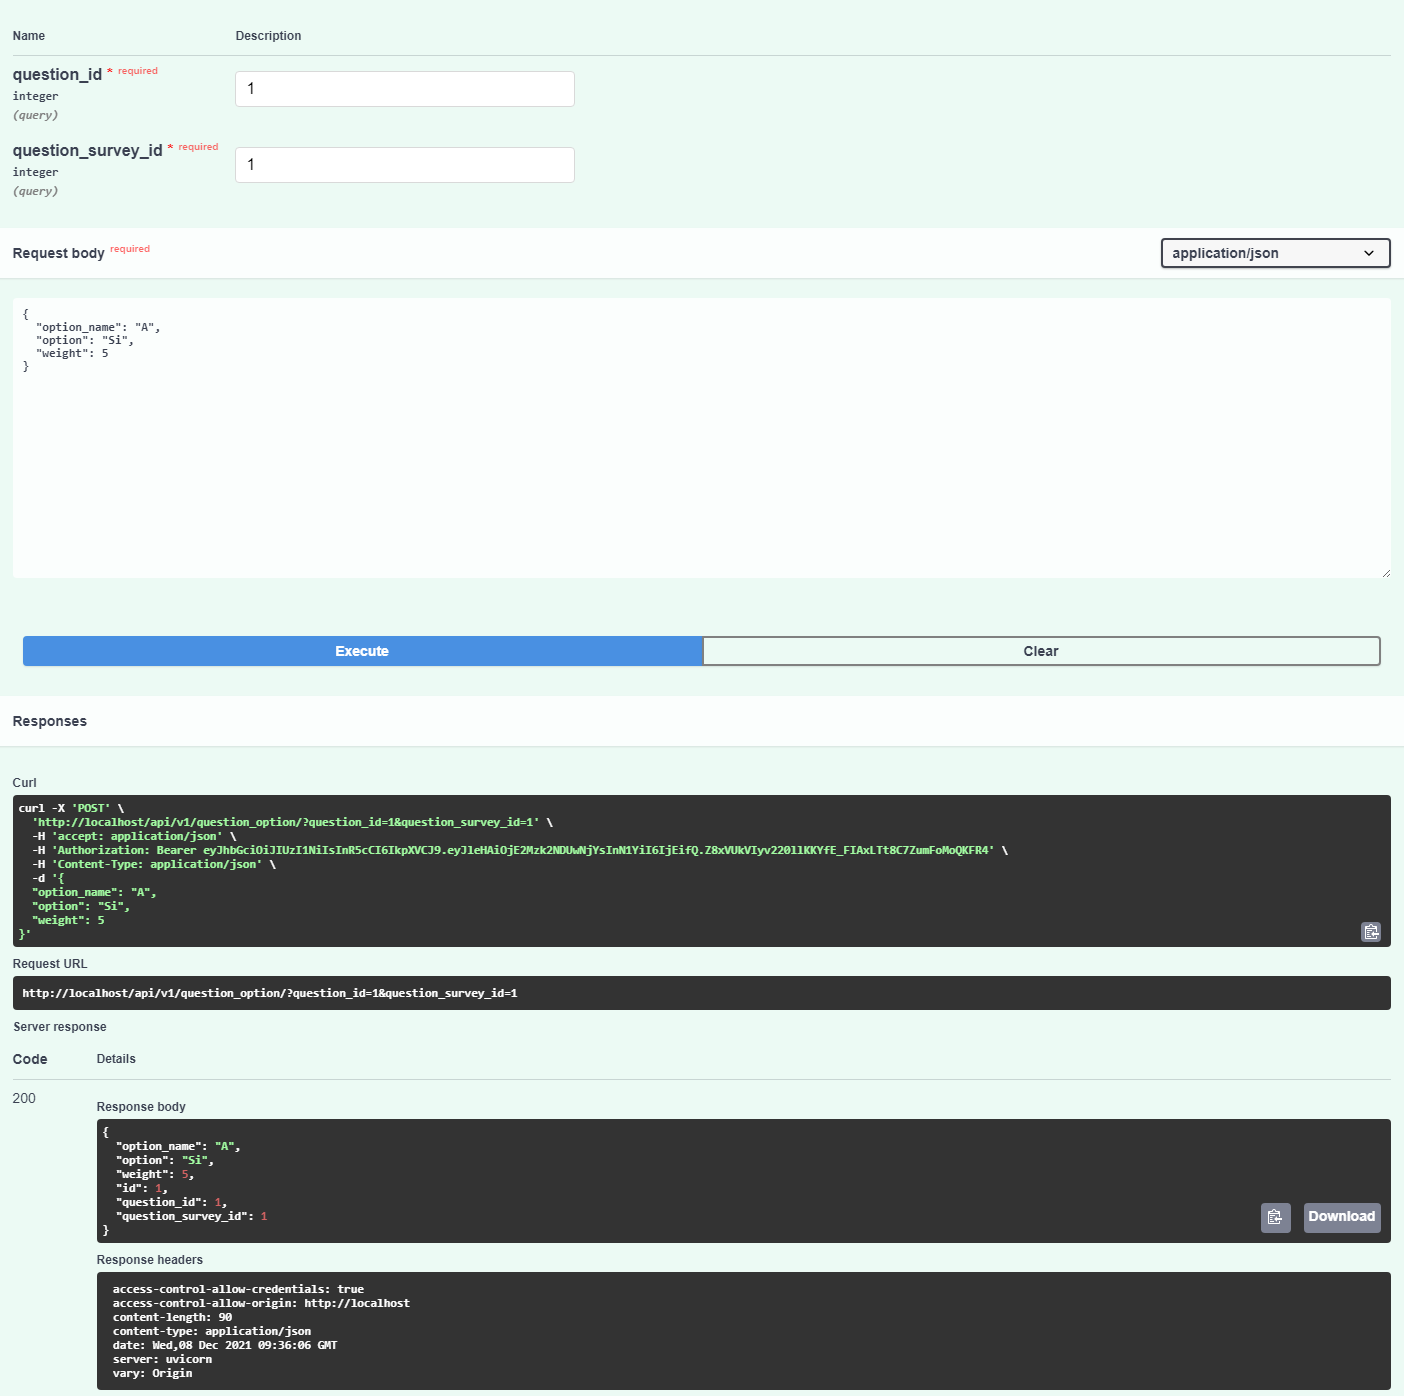
\includegraphics[scale=.3]{TT/img/pruebas/test_crear_opcion_de_respuesta.png}
    \caption{Crear opción de respuesta}
    \label{graphic:crearopcionderespuesta}
\end{figure}

\subsection{Actualizar encuesta}
En la imagen \ref{graphic:actualizarencuesta} se muestra lo necesario para realizar la actualización de una encuesta, esto siempre se debe de realizar cuando sea tenga la primera iteración de preguntas asignadas en la encuesta o se  eliminen preguntas o en su defecto se creen mas, esto se hace para obtener el peso máximo total que tiene la encuesta, con base al numero de preguntas que estén asignadas a la encuesta, también se puede cambiar los mismos campos vistos en la creación de la encuesta. Como resultado ya no se muestra una lista vacía como anteriormente se mostró, si no nos devuelve una lista de las preguntas asignadas junto con sus opciones de respuesta respectivamente.

\begin{figure}[!htb]
    \centering
    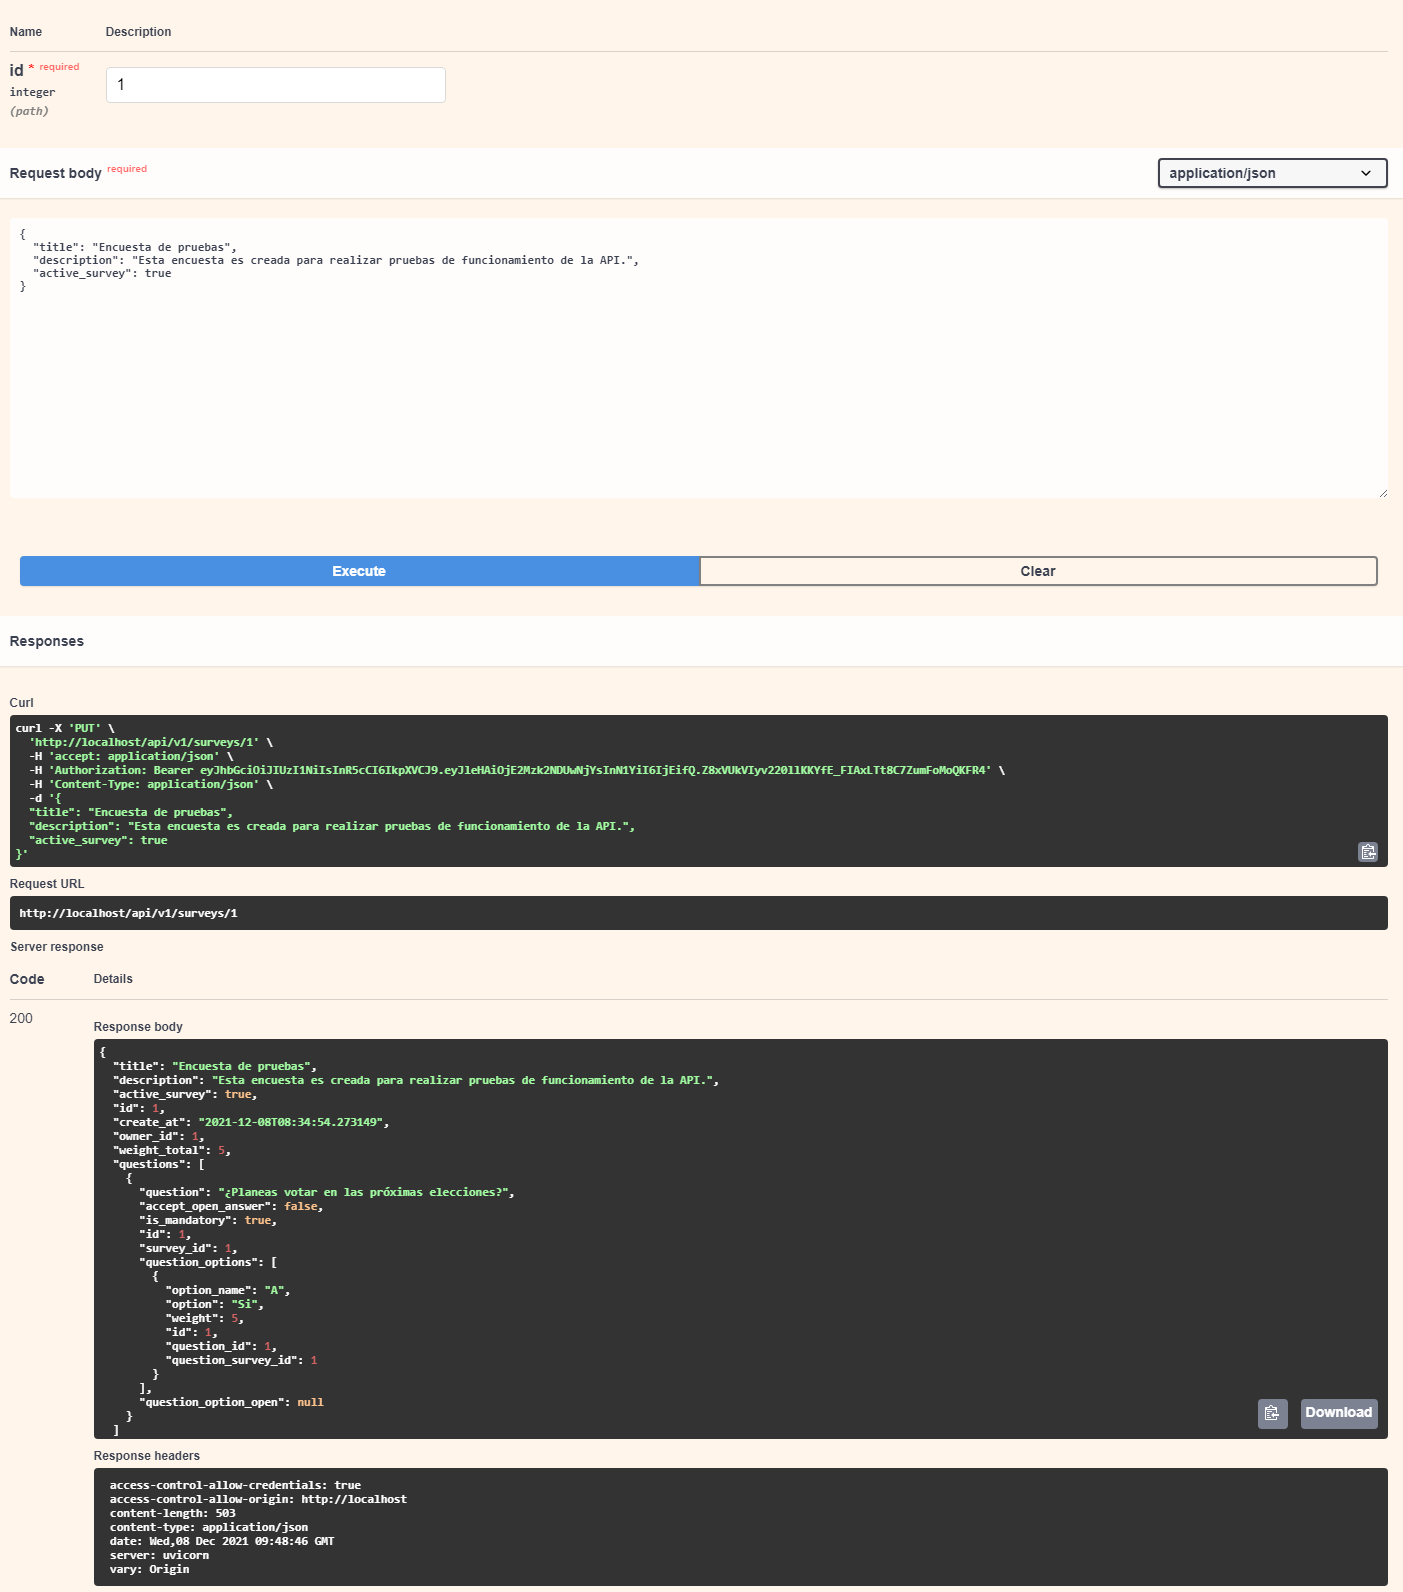
\includegraphics[scale=.3]{TT/img/pruebas/test_actualizar_encuesta.png}
    \caption{Actualizar encuesta}
    \label{graphic:actualizarencuesta}
\end{figure}

\subsection{Crear respuesta}
Por último, en la imagen \ref{graphic:crearrespuesta} se muestra la creación de una respuesta de encuesta. En esta versión del sistema, para guardar una respuesta en la base de datos, es necesario ingresarlas de una en una y al finalizar el ingreso de las respuestas es necesario realizar una petición POST con una URL distinta para realizar un cálculo, este cálculo es para determinar si el usuario '\textit{esta a favor o en contra}' del fin de la encuesta, esto se determina dividiendo la suma obtenida de los pesos elegidos de las respuestas entre el peso máximo total de la encuesta contestada, si es mayor a 0.5 se determina que esta a favor asignado un valor de 1 en una tabla creada exclusivamente para realizar las predicciones, de lo contrario se asigna un 0, esto se muestra en la figura \ref{graphic:crearaceptación}, en esta petición solo hay que enviar el ID de encuesta.

\begin{figure}[!htb]
    \centering
    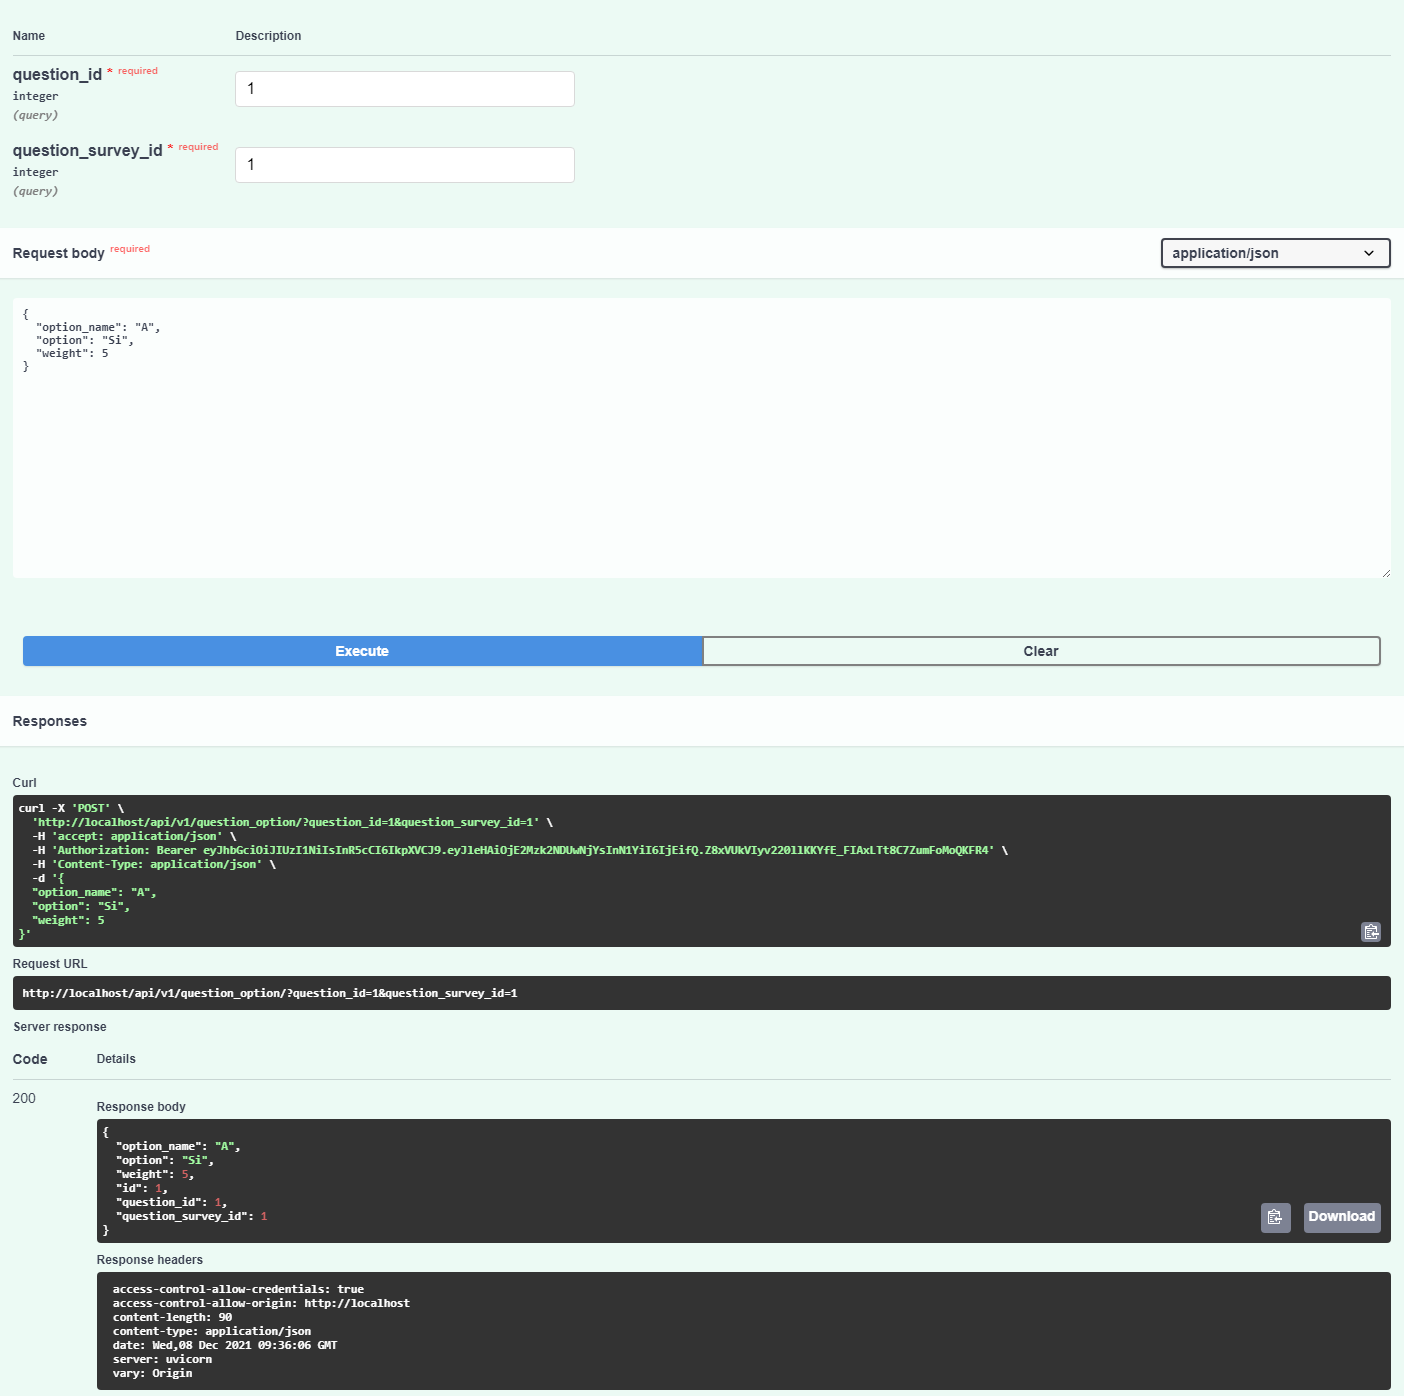
\includegraphics[scale=.3]{TT/img/pruebas/test_crear_opcion_de_respuesta.png}
    \caption{Crear respuesta}
    \label{graphic:crearrespuesta}
\end{figure}

\begin{figure}[!htb]
    \centering
    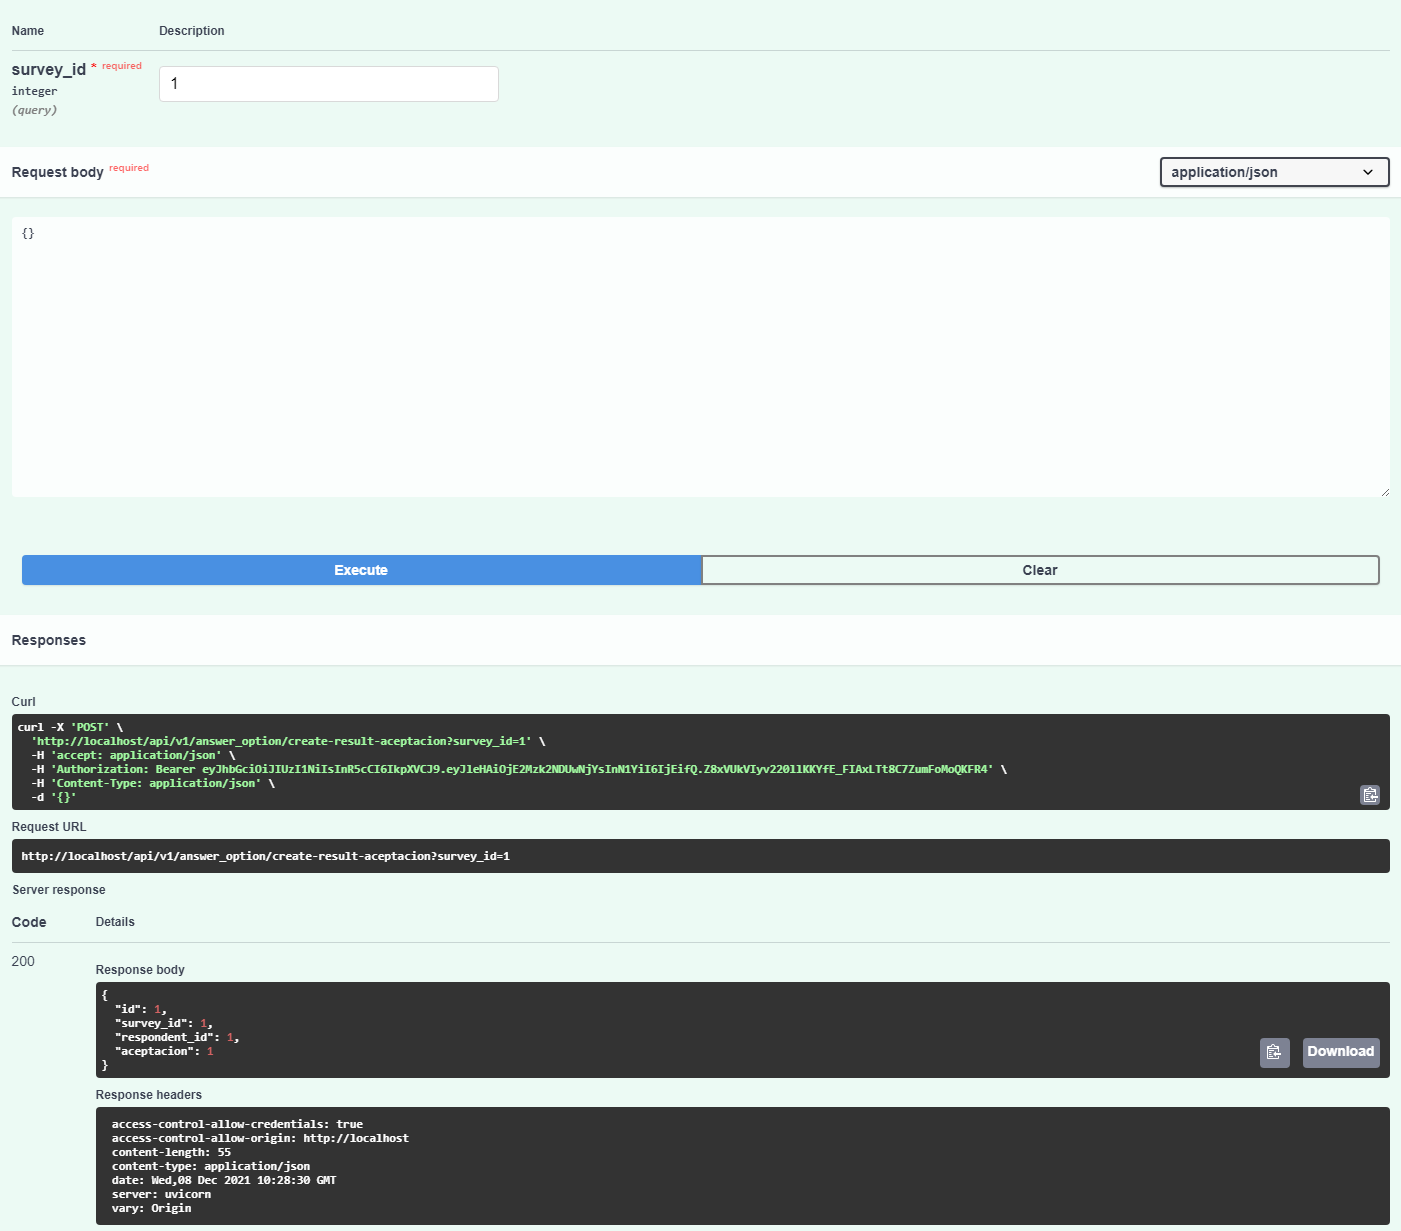
\includegraphics[scale=.3]{TT/img/pruebas/test_crear_aceptacion.png}
    \caption{Crear cálculo de aceptación}
    \label{graphic:crearaceptación}
\end{figure}

\clearpage

\section{Fórmulas usadas para realizar las predicciones}
Algunas de las siguientes ecuaciones se han visto en el capítulo 2, pero se vuelven a presentar en esta sección.

\subsection{Ecuación mágica para grupos de votación de cualquier tamaño}
La siguiente ecuación es propuesta por Serge Galam como función de votación para cualquier el porcentaje de aceptación final y el punto crítico inestable ($p_{c,r}$) para el cálculo de poder total de 'A' o 'B' donde $r >= 4$, siendo r el tamaño del grupo de votación. $m = (r + 1)/2$ para r impar y $m = (r + 1)/2$ para r par para dar cuenta del sesgo favorecido por \textbf{B}. En la imagen \ref{graphic:ecuaciongeneral} se puede mostrar esta ecuación programada en Python.

\begin{equation}
    P_{r}(p_{n}) = \sum_{l=r}^{l=m} \frac{r!}{l!(r-l)!}p_{n}^{l}(1+p_{n})^{r-l},
\end{equation}

\begin{figure}[!htb]
    \centering
    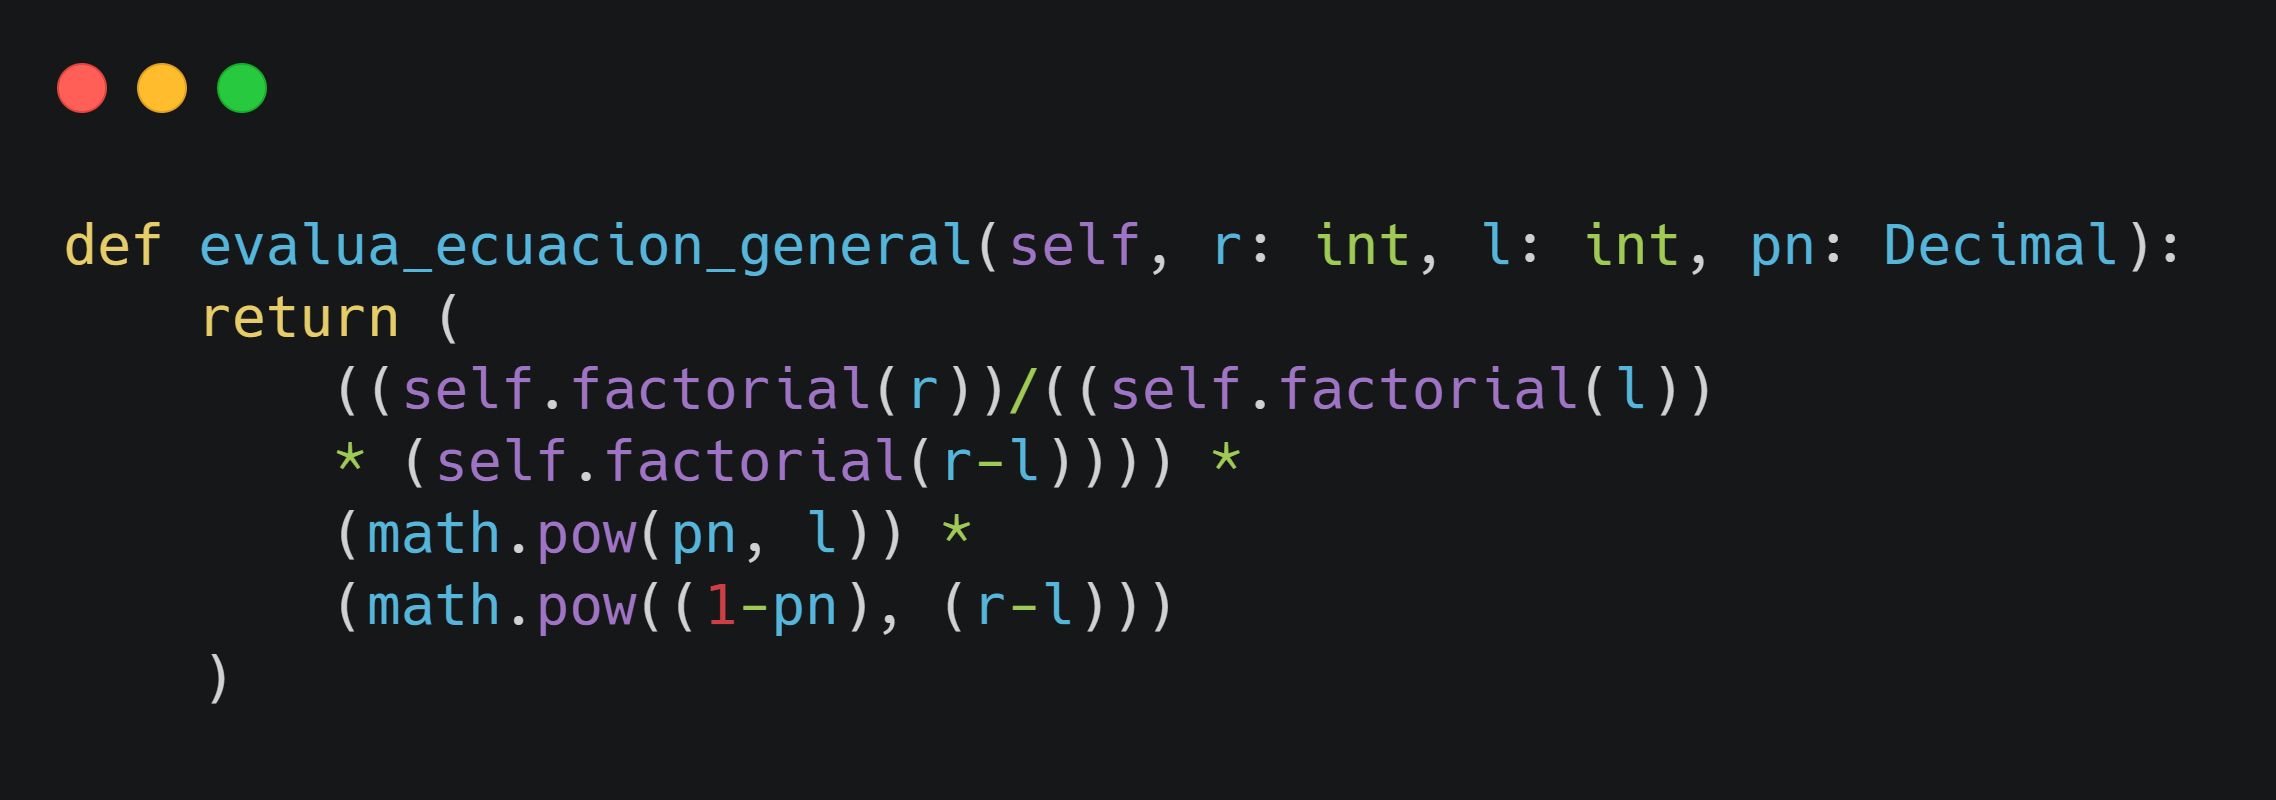
\includegraphics[scale=.15]{TT/img/pruebas/ecuaciongeneral.png}
    \caption{Ecuación general programada}
    \label{graphic:ecuaciongeneral}
\end{figure}

\subsection{Punto crítico inestable}
Galam cálculo los valores de ($p_{c,r}$) hasta $r = 20$, esos valores fueron usados para este proyecto, por lo tanto, para grupos de votación donde $r > 20$ el sistema no funcionará, a continuación se presenta la tabla \ref{table:pcr} con los valores calculados por Galam:

\begin{table}[H]
\centering
\begin{tabular}{cccccccccc}
\rowcolor[HTML]{3166FF} 
{\color[HTML]{FFFFFF} \textit{r}} & {\color[HTML]{FFFFFF} 4} & {\color[HTML]{FFFFFF} 6} & {\color[HTML]{FFFFFF} 8} & {\color[HTML]{FFFFFF} 10} & {\color[HTML]{FFFFFF} 12} & {\color[HTML]{FFFFFF} 14} & {\color[HTML]{FFFFFF} 16} & {\color[HTML]{FFFFFF} 18} & {\color[HTML]{FFFFFF} 20} \\
\textit{$p_{c,r}^{*}$}& 0.77& 0.65 & 0.60& 0.58& 0.56& 0.55& 0.54& 0.54& 0.53                     
\end{tabular}
\caption{Valores de punto fijo inestables en función del tamaño de la celda}
\label{table:pcr}
\end{table}

\subsection{Lambdar}
Otra ecuación necesaria para realizar las predicciones es el calculo de lambdar que esta dada por: 

\begin{equation}
    \lambda_{r} \equiv \left \frac{dP_{r}(p_{n})}{dp_{n}}\right |_{p_{c,r}}
\end{equation}

siendo que $P_{r}(p_{n})$ es la ecuación general o mágica, dando como resultado:

\begin{equation}
    \lambda_{r} = \left \sum_{l=r}^{l=m} \frac{r!}{l!(r-l)!}[p_n^l(r-l)(1-p_n)^{r-l-1}(-1) + (1-p_n)^{r-l}(l)(p_n)^{l-1}]\right |_{p_{c,r}}
\end{equation}

En la imagen \ref{graphic:ecuaciongeneralderivada} se muestra la ecuación general derivada programada en Python y en la imagen \ref{graphic:lambda} la ecuación de lambda.

\begin{figure}[!htb]
    \centering
    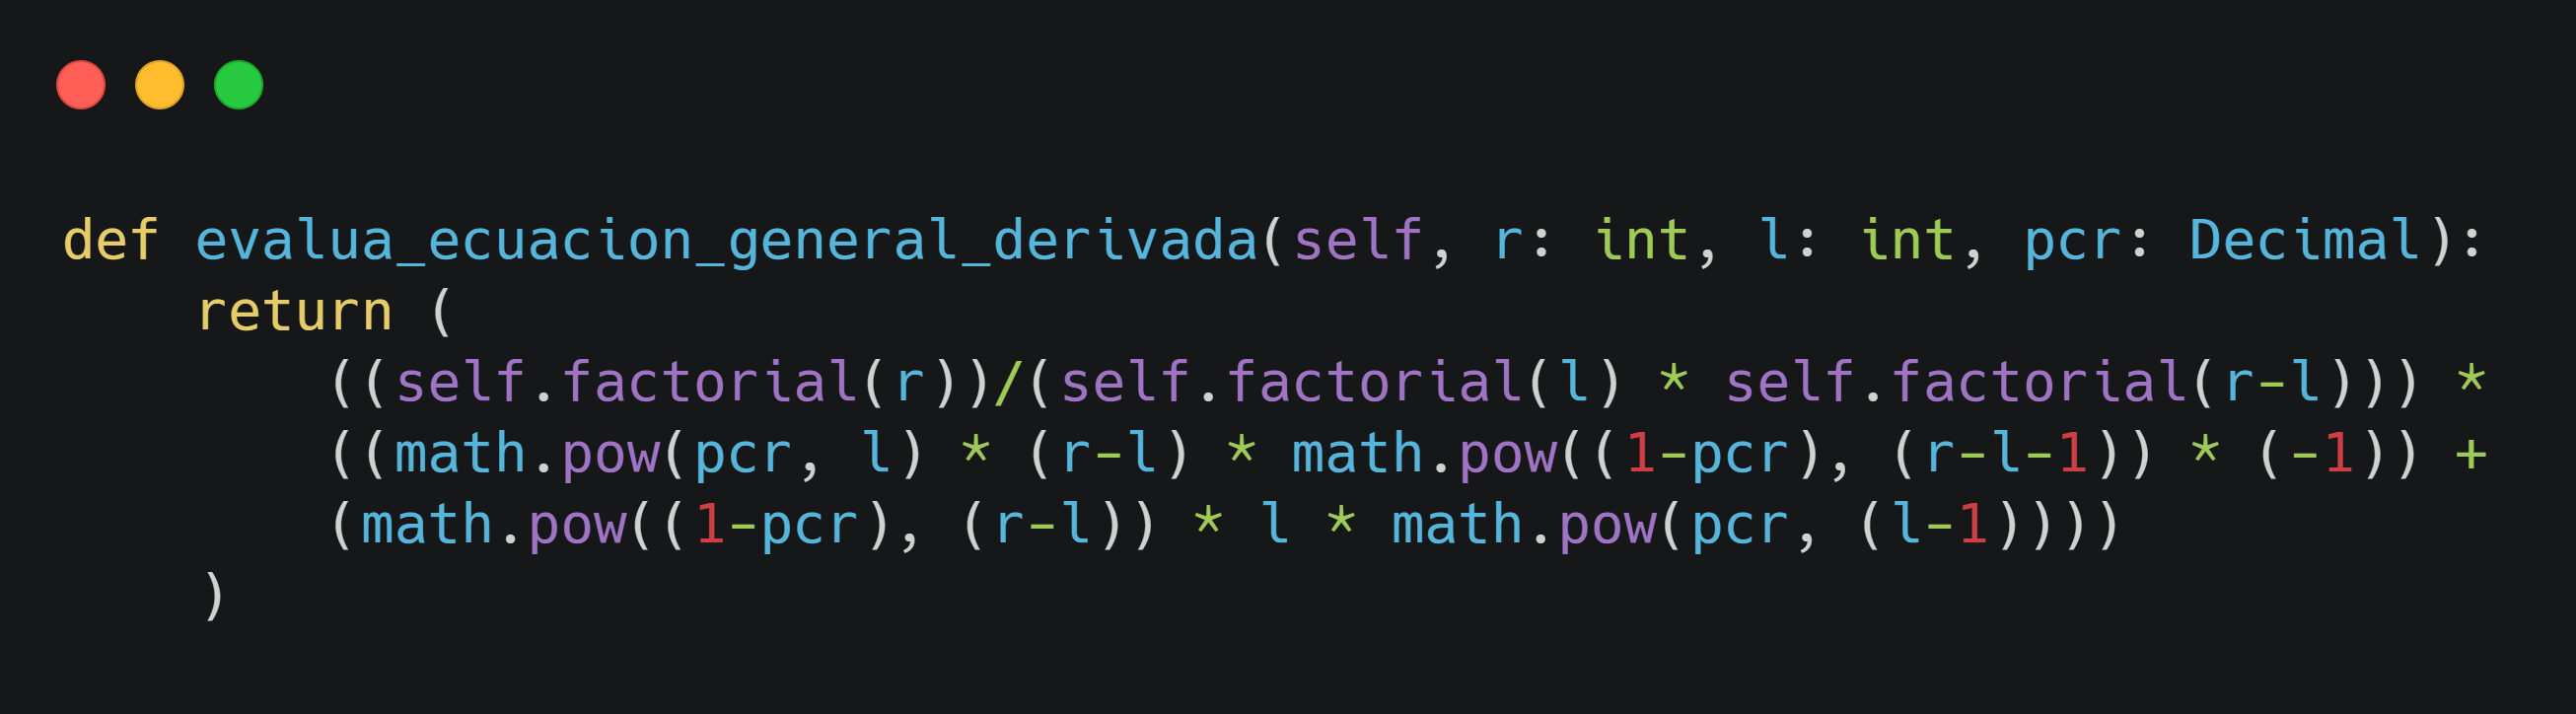
\includegraphics[scale=.15]{TT/img/pruebas/ecuacion_general_derivada.png}
    \caption{Ecuación general derivada programada}
    \label{graphic:ecuaciongeneralderivada}
\end{figure}

\begin{figure}[!htb]
    \centering
    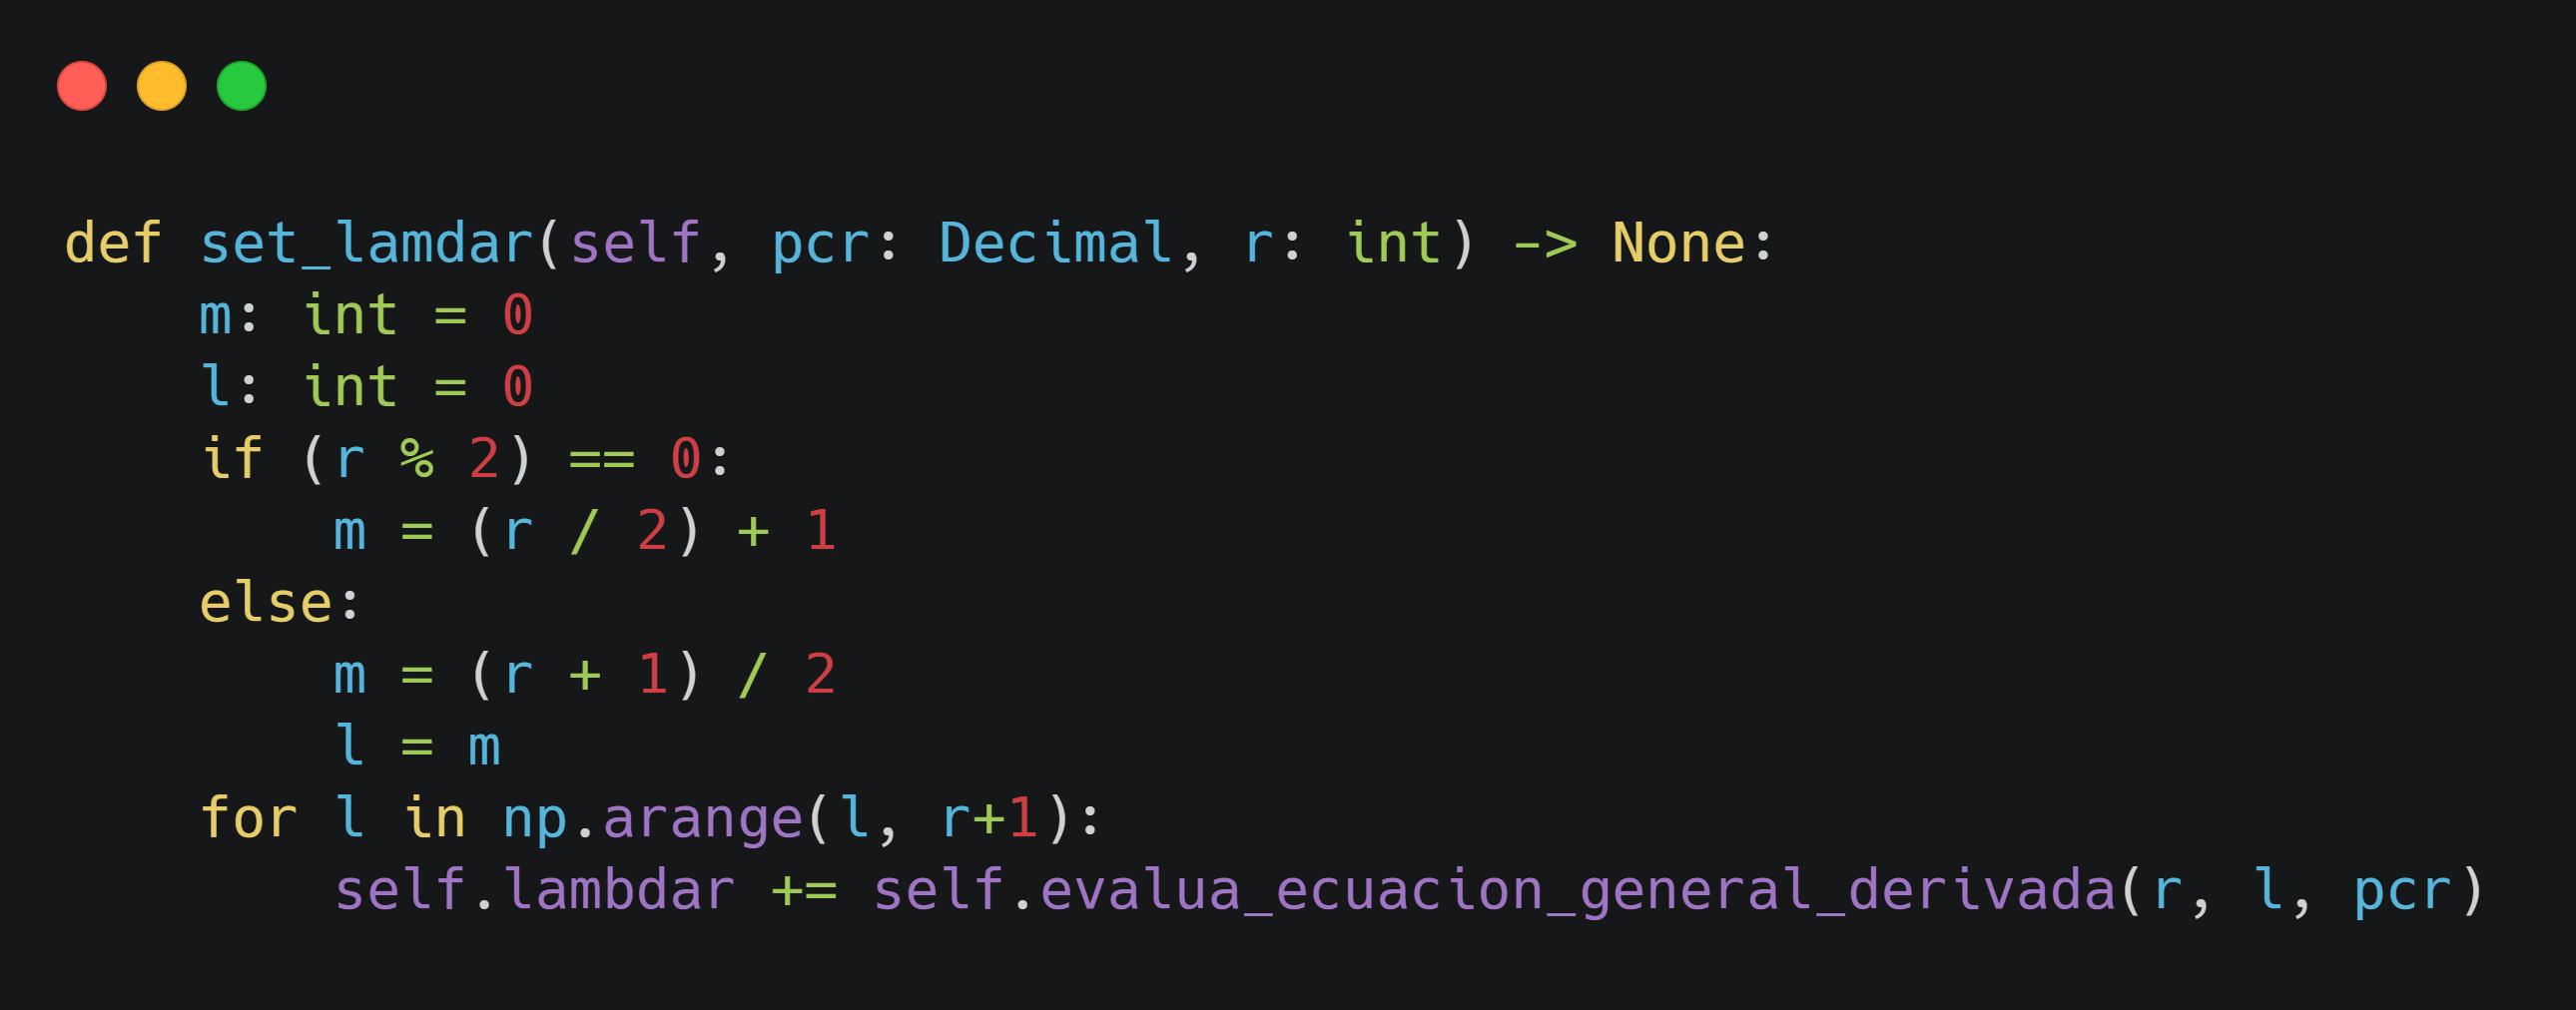
\includegraphics[scale=.15]{TT/img/pruebas/lambda.png}
    \caption{Ecuación de lambda programada}
    \label{graphic:lambda}
\end{figure}

\subsection{Cálculo de porcentaje de victoria y derrota}
Como su nombre lo dice, estas ecuaciones permiten saber que porcentaje mínimo es necesario para asegurar la victoria o derrota y en medio de estos dos datos, se encuentra una región de incertidumbre en donde no se tiene certeza sobre la victoria o derrota. Las ecuaciones son las siguientes:

\subsubsection{Cálculo de porcentaje de derrota}

\begin{equation}
    p_{d,r}^n = p_{c,r}(1-\lambda_r^{-n})
\end{equation}

\begin{figure}[!htb]
    \centering
    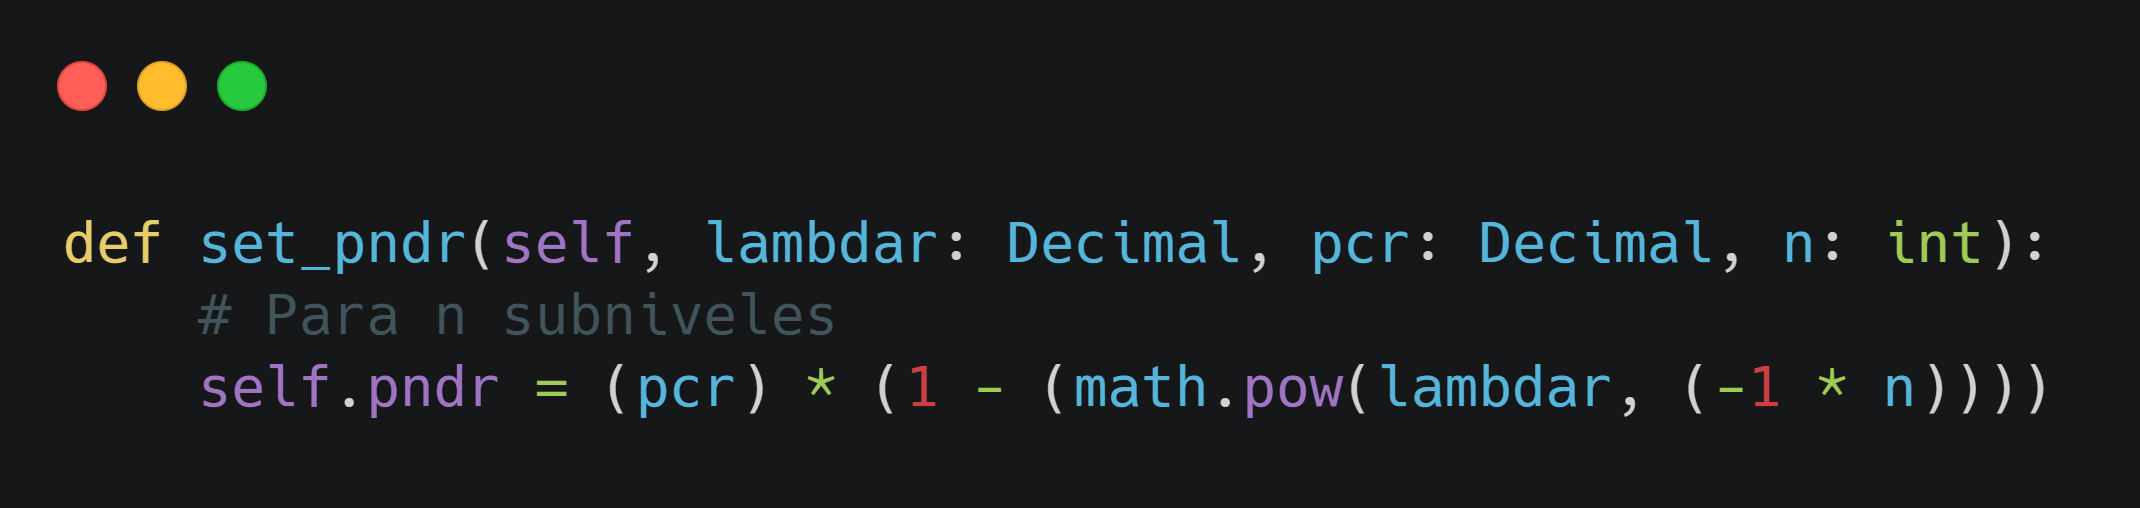
\includegraphics[scale=.15]{TT/img/pruebas/pndr.png}
    \caption{Ecuación de porcentaje de derrota}
    \label{graphic:pndr}
\end{figure}

\subsubsection{Cálculo de porcentaje de victoria}

\begin{equation}
    p_{f,r}^n = p_{d,r}^n + \lambda_r^{-n}
\end{equation}

\begin{figure}[!htb]
    \centering
    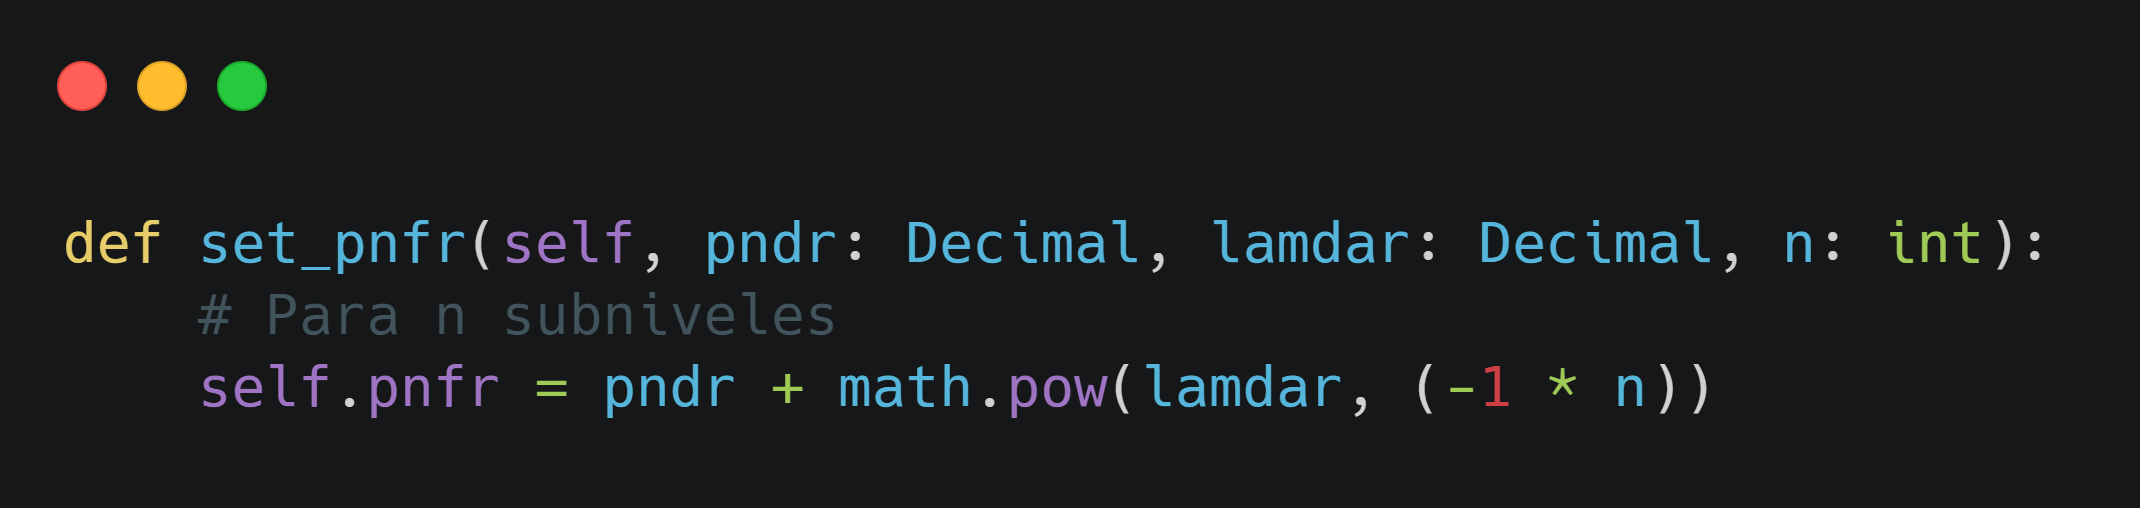
\includegraphics[scale=.15]{TT/img/pruebas/pnfr.png}
    \caption{Ecuación de porcentaje de victoria}
    \label{graphic:pnfr}
\end{figure}

\subsection{Cálculo de aceptación final y de iteraciones para desaparecer}

Para realizar ambos cálculos se resuelven en una misma función. En la imagen \ref{graphic:pn} si $n = -1$ se procede a calcular cuantas iteraciones son necesarias para la eliminación de 'A', si no se pasa ese parámetro, se procede a calcular el porcentaje de aceptación final. Una cosa a destacar, es que se necesita un porcentaje de aceptación inicial menor a 50\% para que el numero de iteraciones sea correcto, de lo contrario, el numero de iteraciones no serán suficientes si el porcentaje es mayor de 50\%.

\begin{figure}[!htb]
    \centering
    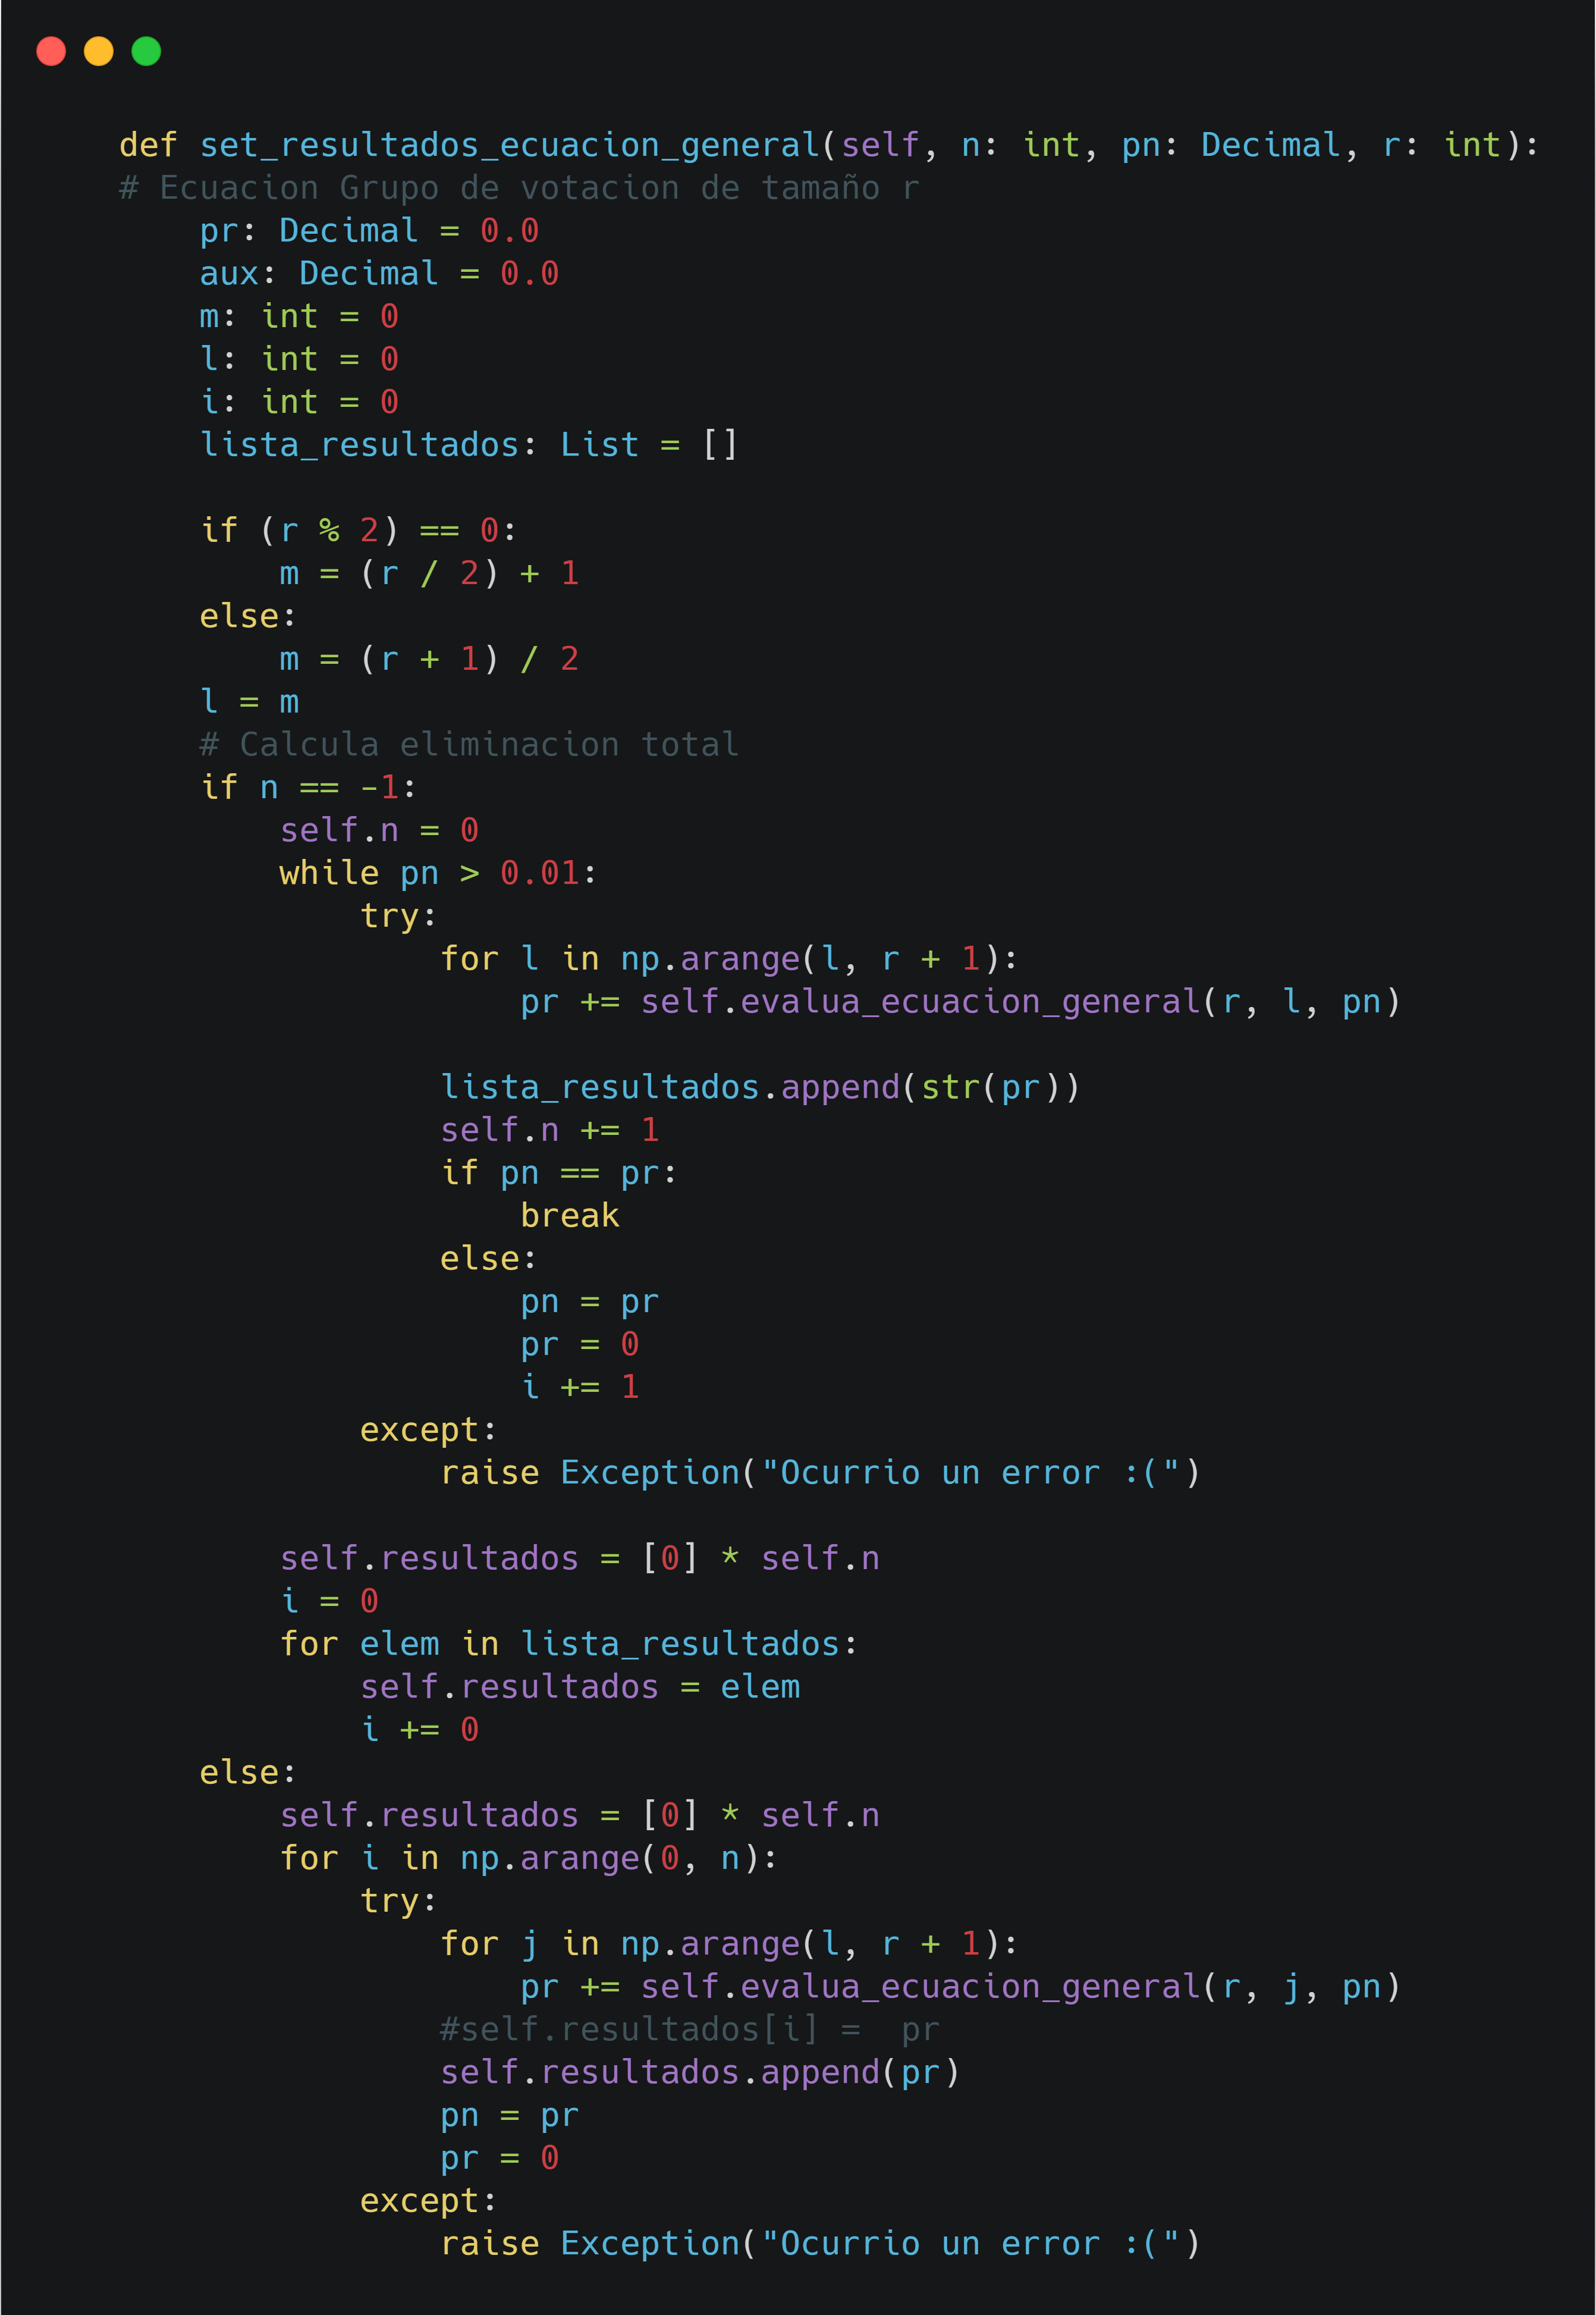
\includegraphics[scale=.15]{TT/img/pruebas/pn.png}
    \caption{Función para calcular el número de iteraciones para la eliminación total y el porcentaje de aceptación final}
    \label{graphic:pn}
\end{figure}

\subsection{Pruebas de resultados de las formulas}
Por último, se presenta una prueba de las formulas descritas anteriormente con base en el artículo de Galam \cite{Galam2008} donde usa los siguientes valores:
\begin{itemize}
    \item $p_0 = 0.69$
    \item $r = 4$
    \item $n = 3$
\end{itemize}

Con lo cual se esperan los siguientes resultados: 
\begin{itemize}
    \item $\lambda \approx 1.64$
    \item $p_{c,4} \approx 0.77$
    \item $p_{d,r}^n \approx 0.59$
    \item $p_{f,r}^n \approx 0.82$
\end{itemize}

En la figura \ref{graphic:testcode} se muestra las líneas de código necesarias para realizar estas pruebas y en la figura \ref{graphic:testresult} se aprecian los resultados entregados de las formulas programadas descritas anteriormente, entregando los resultados acorde al documento de Galam \cite{Galam2008}.
\begin{figure}[!htb]
    \centering
    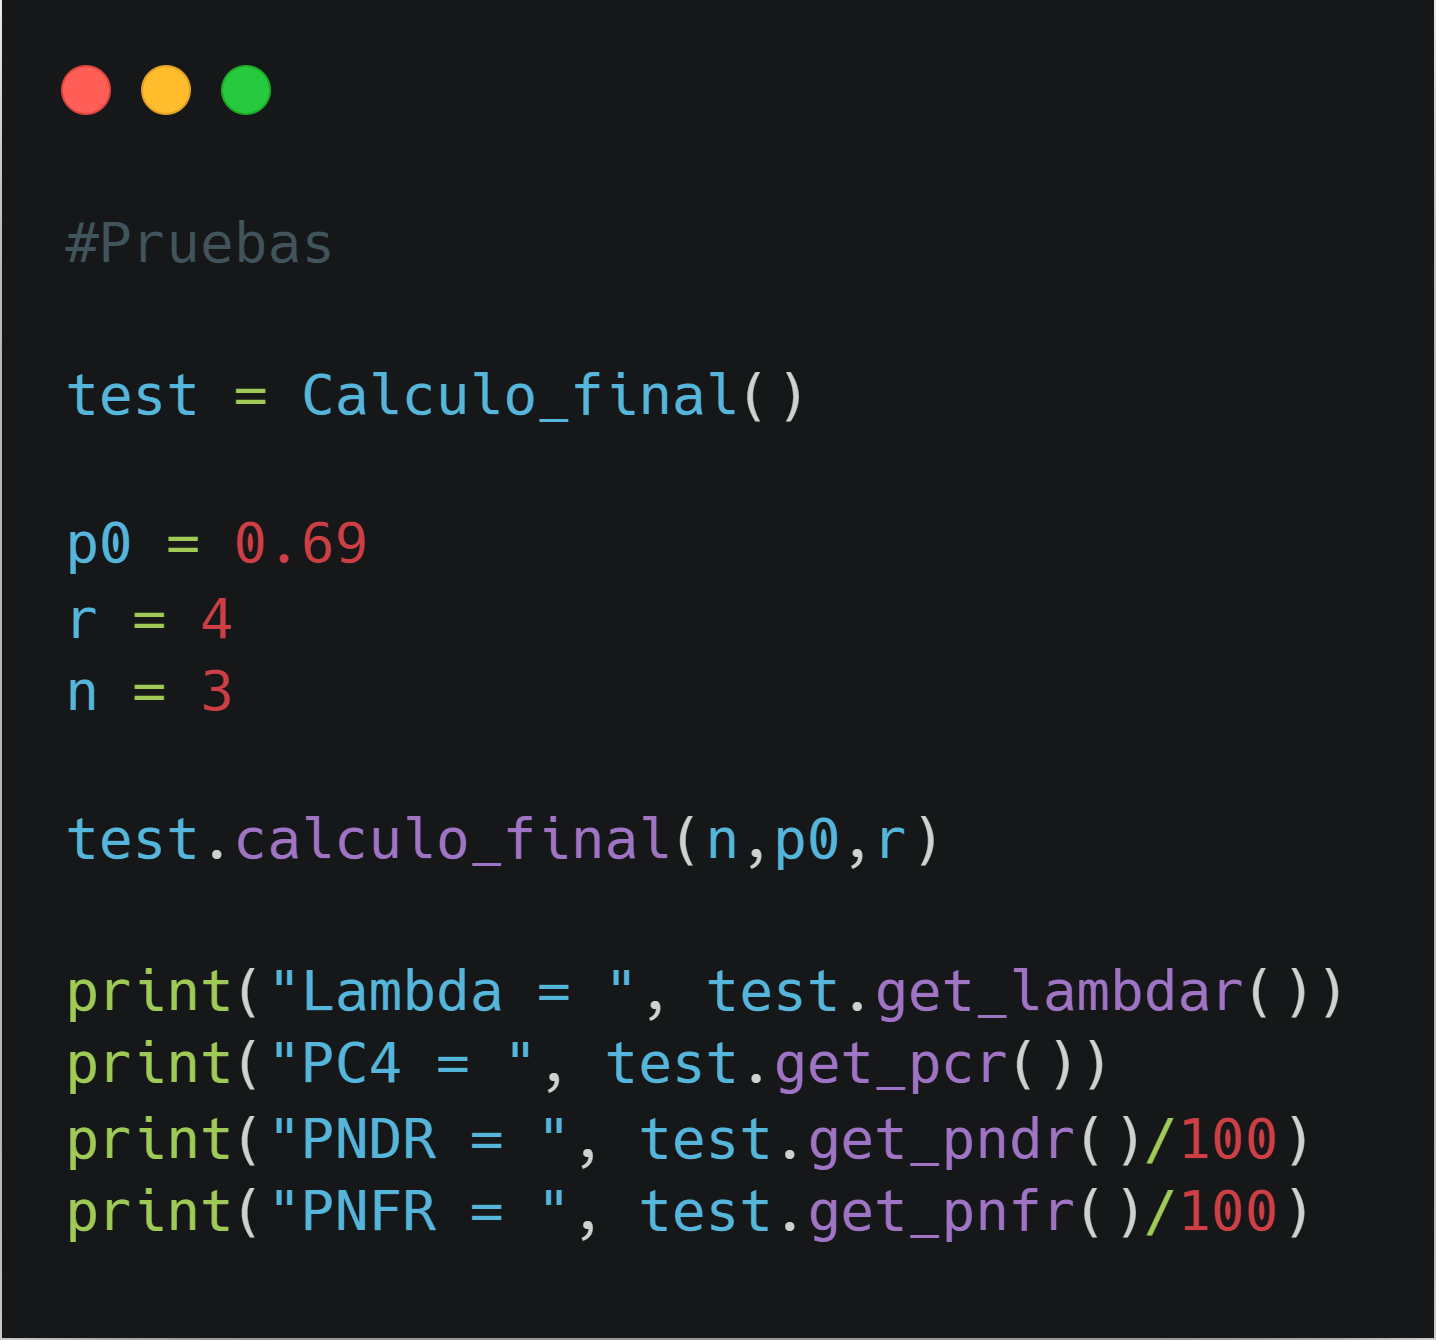
\includegraphics[scale=.25]{TT/img/pruebas/test-formulas.png}
    \caption{Código para probar las fórmulas}
    \label{graphic:testcode}
\end{figure}

\begin{figure}[!htb]
    \centering
    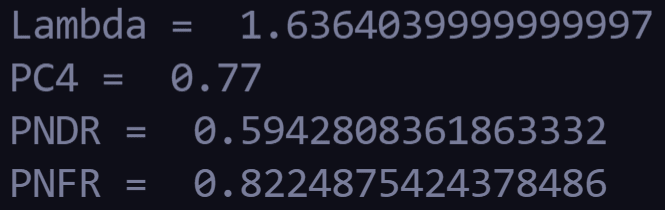
\includegraphics[scale=1]{TT/img/pruebas/test_result.png}
    \caption{Resultados obtenidos de las fórmulas programadas}
    \label{graphic:testresult}
\end{figure}

\clearpage

\section{Validación basada en el artículo 'Sociophysics: A review of Galam Models'}
En dicho artículo se encuentran diversas pruebas realizadas por Serge Galam, en primera instancia realiza una eliminación total de individuos en el sistema, proponiendo los siguientes valores:

\begin{itemize}
    \item Porcentaje inicial: $p_0 = 69$
    \item Tamaño de los grupos votantes: $r = 4$ y toma siete iteraciones para una eliminación total de los adversarios
    \item $p_1 = 63$
    \item $p_2 = 53$
    \item $p_3 = 36$ 
    \item $p_4 = 14$
    \item $p_5 = 1$
    \item $p_6 = 0$
    \item $p_7 = 0$
\end{itemize}

La ejecución se hará en un archivo de Python en el servidor con las formulas descritas anteriormente, dado que SISPREL no guarda la lista final. Esto se hace para que se muestre el resultado en una la imagen \ref{graphic:first_test}.

\begin{figure}[!htb]
    \centering
    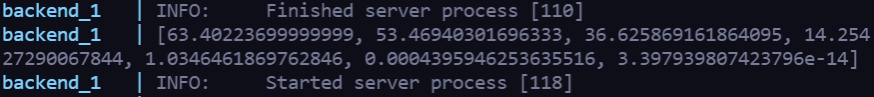
\includegraphics[scale=.9]{TT/img/pruebas/first_test_galam.png}
    \caption{Primera prueba del Artículo 'Sociophysics: A review of Galam Models'}
    \label{graphic:first_test}
\end{figure}

La siguiente prueba es para calcular los umbrales de victoria y derrota, el artículo propone los siguientes datos:
\begin{itemize}
    \item Porcentaje inicial: $p_0 = 69$
    \item Tamaño de los grupos votantes: $r = 4$
    \item $n = 3; PNDR = 59; PNFR = 82$
    \item $n = 4; PNDR = 66; PNFR = 80$
    \item $n = 5; PNDR = 70; PNFR = 79$
\end{itemize}

Para esto haremos uso del punto de acceso '\textit{predictions}' donde se calculan todos los valores descritos anteriormente. En las siguientes imágenes se mostraran únicamente los resultados de los cálculos entregados por SISPREL y en el pie de foto se describirá a que prueba corresponde.

\begin{figure}[!htb]
    \centering
    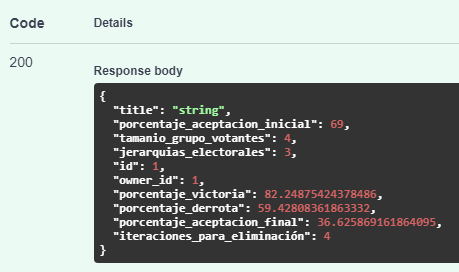
\includegraphics[scale=.9]{TT/img/pruebas/second_test_galam.png}
    \caption{Prueba n = 3}
    \label{graphic:second_test}
\end{figure}

\begin{figure}[!htb]
    \centering
    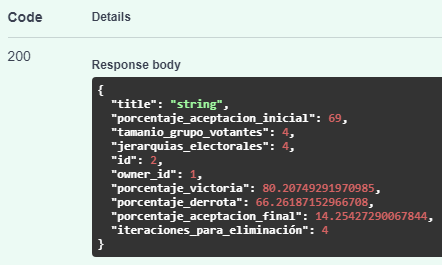
\includegraphics[scale=.9]{TT/img/pruebas/tercera_prueba_galam.png}
    \caption{Prueba n = 4}
    \label{graphic:tercer_test}
\end{figure}

\begin{figure}[!htb]
    \centering
    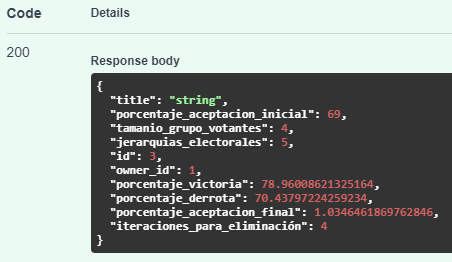
\includegraphics[scale=.9]{TT/img/pruebas/cuarta_prueba_galam.png}
    \caption{Prueba n = 5}
    \label{graphic:cuarto_test}
\end{figure}

Con estas pruebas se ha verificado que el sistema cumple con los resultados calculados por Serge Galam en su artículo 'Sociophysics: A review of Galam Models'.

\clearpage
\section{Validación con datos electorales}
En esta sección pondremos a prueba el sistema con datos del PREP de la Ciudad de México de los años 2015 y 2018, de los cuales solo tomaremos 4 partidos en 3 delegaciones, sin importar quien haya ganado, solo se tomará en cuenta el valor de porcentaje de aceptación final. Se tomarán los resultados de las elecciones de alcaldías del 2015 como porcentaje de aceptación inicial y el objetivo es acercarse a los resultados de las elecciones del 2018, los partidos elegidos son: PRI, PAN, PRD y Morena.

\begin{table}[h]
\centering
\resizebox{15cm}{!} {
\begin{tabular}{m{2.5cm}m{3cm}cccccccc}
\rowcolor[HTML]{3166FF} 
{\color[HTML]{FFFFFF} Partidos\newline Alcaldías} & {\color[HTML]{FFFFFF} Candidato electo} & {\color[HTML]{FFFFFF} PAN} & {\color[HTML]{FFFFFF} MC} & {\color[HTML]{FFFFFF} NA} & {\color[HTML]{FFFFFF} Morena} & {\color[HTML]{FFFFFF} PH} & {\color[HTML]{FFFFFF} ES} & {\color[HTML]{FFFFFF} PRI-PVEM} & {\color[HTML]{FFFFFF} PRD-PT} \\
Azcapotzalco & Pablo Moctezuma (Morena) & 17.07\%  & 2.02\%  & 3.02\%  & 25.70\%  & 2.82\%  & 5.78\%  & 16.44\%  & 20.95\%  \\
Coyoacán & Jose Valentin Maldonado (PRD-PT) & 16.43\%  & 4.15\%  & 1.99\%  & 22.78\%  & 22.92\%  & 4.73\%  & 14.31\%  & 24.96\%  \\
Cuajimalpa de Morelos & Miguel Angel Salazar (PRI-PVEM) & 24.70\%  & 1.05\%  & 1.16\%  & 9.86\%  & 1.58\%  & 2.13\%  & 33.70\% & 17.75\%  \\
G.A.M & Victor Hugo Lobo (PRD-PT)& 11.33\%  & 3.71\%  & 3.03\%  & 24.79\%  & 2.31\%  & 5.24\%  & 14.35\%  & 25.03\% 
\end{tabular}
}
\caption{Resultados de elecciones del 2015. \cite{IEDF2015}}
\label{table:Elecciones2015}
\end{table}

\begin{table}[h]
\centering
\resizebox{15cm}{!} {
\begin{tabular}{m{2.5cm}m{3cm}cccccc}
\rowcolor[HTML]{3166FF} 
{\color[HTML]{FFFFFF} Partidos \newline Alcaldías} & {\color[HTML]{FFFFFF} Ganador} & {\color[HTML]{FFFFFF} PAN-PRD-MC} & {\color[HTML]{FFFFFF} PRI} & {\color[HTML]{FFFFFF} PVEM} & {\color[HTML]{FFFFFF} Morena-PT-ES} & {\color[HTML]{FFFFFF} NA} & {\color[HTML]{FFFFFF} ES} \\
Azcapotzalco & MORENA-PT-ES & 33.24\% & 8.11\% & 3.16\% & 49.67\% & 1.25\% & 1.95\% \\
Coyoacán & PAN-PRD-MC & 45.97\% & 9.36\% & 3.09\% & 34.85\% & 1.72\% & 2.14\% \\
Cuajimalpa de Morelos & PRI & 27.86\% & 37.12\% & 1.94\% & 28.64\% & 1.11\%& 1.01\% \\
G.A.M & MORENA-PT-ES & 29.79\% & 9.05\% & 4.36\% & 48.88\% & 2.18\% & 2.71\%
\end{tabular}
}
\caption{Resultados de elecciones del 2018. \cite{IECM2018}}
\label{table:Elecciones 2018}
\end{table}

\begin{figure}[!htb]
    \centering
    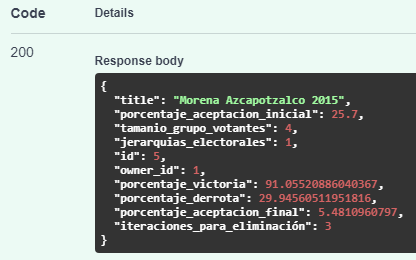
\includegraphics[scale=.5]{TT/img/pruebas/Morena Azcapotzalco 2015.png}
    \caption{Predicción para el partido Morena en Azcapotzalco para 2018}
    \label{graphic:MORENAAZC2015}
\end{figure}

\begin{figure}[!htb]
    \centering
    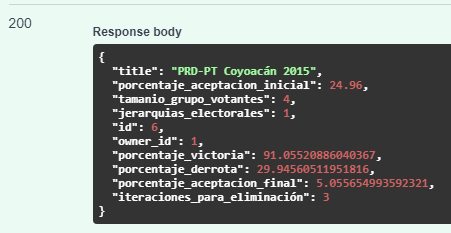
\includegraphics[scale=.5]{TT/img/pruebas/PRD-PT Coyoacan 2015.png}
    \caption{Predicción para la coalición PRD-PT en Coyoacán para 2018}
    \label{graphic:PRDPTCOY2015}
\end{figure}

\begin{figure}[!htb]
    \centering
    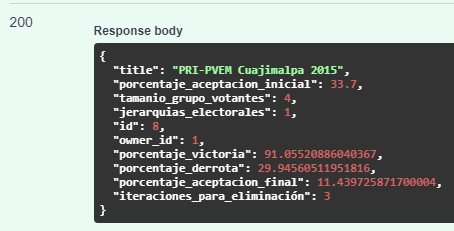
\includegraphics[scale=.5]{TT/img/pruebas/PRI-PVEM Cuajimalpa 2015.png}
    \caption{Predicción para la coalición PRI-PVEM en Cuajimalpa para 2018}
    \label{graphic:PRIPVEM2015}
\end{figure}

\begin{figure}[!htb]
    \centering
    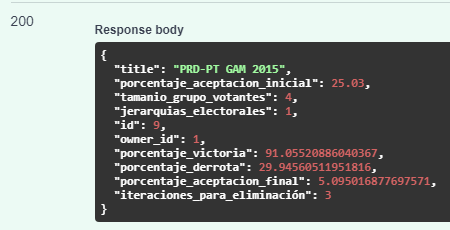
\includegraphics[scale=.5]{TT/img/pruebas/PRD-PT GAM 2015.png}
    \caption{Predicción para la coalición PRD-PT en la GAM para 2018}
    \label{graphic:PRDPT2015}
\end{figure}


Se tomaron los valores iniciales del 2015 por delegación tomando en cuenta al ganador como el porcentaje de aceptación inicial, el tamaño de grupos de votantes se toma como 4 dado que se han analizado solo 4 delegaciones. En las imágenes \ref{graphic:MORENAAZC2015}, \ref{graphic:PRDPTCOY2015}, \ref{graphic:PRIPVEM2015} y \ref{graphic:PRDPT2015} se encuentran resultados muy distintos a lo que sucedió realmente en las elecciones del 2018, pero esto puede tener una explicación, las predicciones han errado pero se debe a que se realizaron para una coalición en especifico y en la elección siguiente ya no estaban porque se dividieron y se aliaron con otros partidos. También se puede apreciar que al menos un partido de las coaliciones del 2015 que estaban en el poder continuaron en el poder en las elecciones del 2018 de los cuales Morena, PT, PRD y el PRI continuaron con el poder en sus respectivas alcaldías pero con diferentes aliados.

Dado que los primeros datos propuestos no logramos tener un porcentaje de error conciso, realizaremos una segunda prueba pero tomando como referencia los del año 2006 y 2008 donde aun se mantenían de manera mas estables, las coaliciones entre partidos. 

\begin{table}[h]
\centering
\resizebox{15cm}{!} {
\begin{tabular}{m{2.5cm}m{3cm}ccccc}
\rowcolor[HTML]{3166FF} 
{\color[HTML]{FFFFFF} Partido\newline Delegacion} & {\color[HTML]{FFFFFF} Candidato electo} & {\color[HTML]{FFFFFF} PAN} & {\color[HTML]{FFFFFF} PRI-PVEM} & {\color[HTML]{FFFFFF} PRD-PT-CONV} & {\color[HTML]{FFFFFF} NA} & {\color[HTML]{FFFFFF} PASC} \\
Azcapotzalco & Alejandro Carvajal (PRD-PT-CONV) & 33.63\% & 13.40\%\% & 45.99\% & 3.63\% & 1.43\% \\
Coyoacán & Antonio Heberto Castillo (PRD-PT-CONV) & 30.41\% & 11.68\% & 50.14\% & 4.20\% & 2.20\% \\
Cuajimalpa & Remedios Ledezma García (PRD-PT-CONV) & 27.49\% & 18.94\% & 37.01\% & 12.12\% & 2.52\% \\
GAM & Francisco Chiqui (PRD-PT-CONV) & 23.02\% & 12.21\% & 54.84\% & 5.88\% & 2.43\%
\end{tabular}
}
\caption{Resultados de elecciones del 2006. \cite{IECM2006}}
\label{table:Elecciones2006}
\end{table}

\begin{table}[h]
\centering
\resizebox{15cm}{!} {
\begin{tabular}{m{2.5cm}m{3cm}llllllllm{2cm}m{2cm}}
\rowcolor[HTML]{3166FF} 
{\color[HTML]{FFFFFF} Partido\newline Delegacion} & {\color[HTML]{FFFFFF} Candidato electo} & {\color[HTML]{FFFFFF} PAN} & {\color[HTML]{FFFFFF} PRI} & {\color[HTML]{FFFFFF} PRD} & {\color[HTML]{FFFFFF} PT} & {\color[HTML]{FFFFFF} PVEM} & {\color[HTML]{FFFFFF} CONV} & {\color[HTML]{FFFFFF} NA} & {\color[HTML]{FFFFFF} PSD} & {\color[HTML]{FFFFFF} PRD-PT-CONV} & {\color[HTML]{FFFFFF} PRD-CONV} \\
Azcapotzalco & Enrique Vargas (PRD-CONV) & 25.29\% & 17.10\% & 30.00\% & 3.63\% & 1.43\% & 1.75\% & 3.09\% & 1.10\% &  & 1.01 \\
Coyoacán & Raul Antonio Flores (PRD-PT-CONV) & 28.98\% & 13.62\% & 29.34\% & 6.65\% & 5.04\% & 1.50\% & 2.37\% & 1.44\% & 1.65 &  \\
Cuajimalpa & Carlos Orvañanos (PAN) & 41.24\% & 11.34\% & 29.24\% & 2.34\% & 3.02\% & 0.70\% & 3.30\% & 0.94\% & 1.92\% &  \\
GAM & Victor Hugo Lobo Román (PRD) & 17.96\% & 16.38\% & 35.09\% & 6.47\% & 7.33\% & 2.51\% & 3.26 \%& 1.30\% &  & 
\end{tabular}
}
\caption{Resultados de elecciones del 2009. \cite{IEDF2009}}
\label{table:Elecciones2015}
\end{table}

Realizamos la misma prueba tomando al alcalde electo y su respectivo porcentaje de su coalición para realizar tomarlo como porcentaje de aceptación inicial, el numero que consiste el grupo de votantes es de 4 por las 4 delegaciones que han sido escogidas y un numero de jerarquías electorales porque se realiza solo un conteo. A continuación se realizará el cálculo de un partido político y los demás resultados se mostrarán en una tabla, comparando los resultados obtenidos con los de la elección del 2009.

El ejemplo a realizar toma los datos de Enrique Vargas, alcalde electo de la alcaldía de Azcapotzalco con la coalición PRD-CONV. A continuación los datos para realizar los cálculos:

\begin{itemize}
    \item $p_0 = 45.99\%$
    \item $r = 4$
    \item $n = 1$
\end{itemize}

El resultado se muestra en la imagen \ref{graphic:PRDPTCONV2006}.
\begin{figure}[!htb]
    \centering
    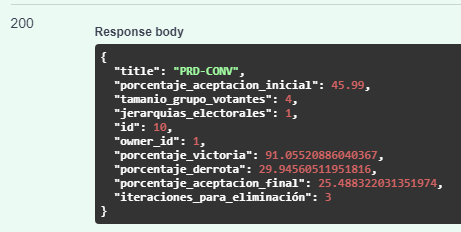
\includegraphics[scale=.5]{TT/img/pruebas/PRD-CONV AZC 2006.png}
    \caption{Predicción para la coalición PRD-PT-CONV en la alcaldía Azcapotzalco para 2009}
    \label{graphic:PRDPTCONV2006}
\end{figure}

De esta manera, obtenemos un porcentaje de aceptación final de 25.48\% aprox. proveniente de SISPREL. En la siguiente tabla se muestran los resultados obtenidos comparados con los de la elección del 2006, en el 2009 hubo algunos partidos que se salieron de la coalición, pero como no se aliaron, estos se suman a la coalición que mantuvo 2 de los 3 partidos que estaban juntos en las elecciones del 2006.

\begin{table}[H]
\centering
\begin{tabular}{|l|l|l|l|}
\hline
\rowcolor[HTML]{3166FF} 
{\color[HTML]{FFFFFF} Aceptación en 2006} & {\color[HTML]{FFFFFF} Predicción a 2009} & {\color[HTML]{FFFFFF} Aceptación en 2009} & {\color[HTML]{FFFFFF} \% de error} \\ \hline
45.99\% & 25.48\% & 32.75\% & 7.27\% \\ \hline
50.14\% & 31.46\% & 39.14\% & 7.68\% \\ \hline
37.01\% & 14.64\% & 41.23\% & 26.59\% \\ \hline
54.84\% & 38.83\% & 35.08\% & 3.75\% \\ \hline
\end{tabular}
\caption{Comparación entre predicción y datos reales. }
\label{table:resultadosprediccion}
\end{table}

El promedio de error realizado en este análisis real se tiene un promedio de 11.3\%, cumpliendo con la tolerancia de error del 30\% planteado en el análisis, por lo tanto el sistema es confiable.